\documentclass[11pt, a4paper]{article}

\usepackage{palatino}
\usepackage{amsmath, amssymb, amsthm}
\usepackage{geometry}
\usepackage{microtype}
\usepackage{hyperref}
\usepackage{setspace}
\usepackage{csquotes}
\usepackage{titlesec}
\usepackage{abstract}
\usepackage{natbib}
\usepackage{tikz}
\usetikzlibrary{arrows.meta,positioning,calc,fit}
\usepackage{graphicx}

\geometry{
  top=1.25in,
  bottom=1.25in,
  left=1.25in,
  right=1.25in
}

\onehalfspacing

\hypersetup{
  colorlinks=true,
  linkcolor=black,
  citecolor=black,
  urlcolor=black
}

\titleformat{\section}{\large\bfseries}{\thesection.}{0.75em}{}
\titleformat{\subsection}{\normalsize\bfseries}{\thesubsection.}{0.75em}{}

\theoremstyle{plain}
\newtheorem{theorem}{Theorem}
\newtheorem{proposition}{Proposition}
\newtheorem{lemma}{Lemma}
\newtheorem{corollary}{Corollary}
\theoremstyle{definition}
\newtheorem{definition}{Definition}
\theoremstyle{remark}
\newtheorem{remark}{Remark}

%% Shorthand
\newcommand{\simA}{\sim_A}
\newcommand{\simO}{\sim_O}
\newcommand{\simC}{\sim_C}
\newcommand{\simI}{\sim_I}
\newcommand{\RHP}{\mathcal{R}_H^\Pi}
\newcommand{\DA}{D_A(\varphi)}

\title{%
  \textbf{Against Latent Fundamentalism}\\[0.5em]
  {\large\itshape Admissibility Distortion and the Missing Criterion\\
  in Representation Learning for Planning}%
}

\author{Flyxion\\
\small Independent Researcher}

\date{\today}

\begin{document}

\maketitle

\begin{abstract}
\noindent
Representation learning for planning is missing a fundamental criterion. Planning
requires distinguishing states that differ in which futures are accessible; this
requirement induces the admissibility equivalence relation~$\simA$ as the coarsest
relation compatible with adequate planning, and correspondingly induces a
canonical measure of representational failure: the admissibility distortion
$\DA$, equal to zero if and only if the learned projection is admissibility-preserving.
The paper's central theorem---the Observational--Interventional Separation
Theorem---establishes that observational equivalence does not imply interventional
equivalence, $\simO \not\Rightarrow \simI$, and identifies this as a category
mismatch rather than an empirical contingency: observation generates equivalence
classes over distributions while intervention generates equivalence classes over
reachability geometry. Three corollaries follow immediately: predictive projections
satisfy $D_A(\varphi_P) \not\equiv 0$ in general; compressive projections satisfy
$D_A(\varphi_C) \not\equiv 0$ in general; and any guardrail classifier operating
on a projection with $\DA > 0$ is subject to irrecoverable failure on the
collapsed distinctions. The last result is derived from the data-processing
inequality as a general bound, with the zero-information case yielding a complete
impossibility theorem. Every existing approach to representation learning can be
understood as proposing a candidate quotient space; the admissibility question
asks how far that proposal departs from the quotient planning requires.
Recent work questioning whether world models constitute understanding
\citep{gupta2025world} converges on a related diagnosis from a philosophical
direction; the present paper proposes admissibility distortion as a candidate
formal quantity underlying the representational failures such analyses identify. Recent advocacy for Joint
Embedding Predictive Architectures motivates the inquiry but does not determine
its scope. The contribution is the identification of admissibility distortion
as a quantity that representation learning currently lacks the means to measure,
bound, or regularise.
\end{abstract}

\newpage

\section{Introduction}

Planning requires choosing among actions by evaluating their consequences. This
simple observation has a non-trivial mathematical implication: any representation
intended to support planning must preserve, at minimum, the distinctions that
determine which futures are accessible from which states. When a representation
fails to preserve such distinctions, planning errors follow that cannot be
corrected by improving the optimiser, refining the cost function, or adding
architectural safety machinery. The failure is prior to all of those operations.

Despite this, representation learning for planning currently lacks a principled
criterion for evaluating whether a learned projection preserves the distinctions
planning requires. The objectives in widespread use---predictive accuracy,
information maximisation, compression progress, contrastive separation---optimise
for properties of the observation distribution. None of them directly optimise
for preservation of reachability structure. The question of whether a given
latent space is adequate for planning is therefore not directly addressed by
any current training objective; it is at most hoped that predictive or compressive
representations will be adequate incidentally.

The missing criterion is admissibility distortion, denoted
$\DA$, and that the prior condition for its use is the admissibility equivalence
relation $\simA$ derived from the requirements of planning itself. The argument
has a specific logical architecture. Planning induces $\simA$ and thereby induces
$\DA$. Prediction and compression are then understood not as competitors to
admissibility but as proposals for constructing admissibility-preserving quotient
spaces, evaluated by the question $\simO \stackrel{?}{\approx} \simA$ and
$\simC \stackrel{?}{\approx} \simA$. The paper's results establish that both
proposals fail in general---that $D_A(\varphi_P) \not\equiv 0$ and
$D_A(\varphi_C) \not\equiv 0$---and that the failure is structural rather than
incidental. An information-theoretic consequence follows immediately: admissibility
information destroyed by projection cannot be recovered by any downstream
computation.

A parallel critique has recently been advanced on philosophical grounds.
\citet{gupta2025world} argue, through case studies drawn from Hofstadter, Poincar\'e,
and Popper, that world models fail to capture human understanding because
state-tracking and state-transition simulation are insufficient for understanding
the explanatory structure that governs a system. Their core objection---that
mechanistic simulation of states does not yield the organising principles that
make those states significant---runs parallel to the admissibility critique, and
the two converge on a structurally similar conclusion. The present paper provides
the formal criterion that philosophical critiques of this kind implicitly require:
the quantity that world models fail to preserve is admissibility distortion, the
departure of a learned quotient from the quotient that planning and understanding
jointly require. This connection is developed at the relevant points throughout.

Recent articulation of Joint Embedding Predictive Architectures (JEPA) as the
proper foundation for artificial general intelligence motivates the inquiry by
making the underlying assumption unusually explicit: that self-supervised latent
representations learned by predicting masked video constitute sufficient state
descriptions for planning and safe action. Examining this claim carefully reveals
that the assumption is not established by the empirical record, but more
importantly reveals that the criterion by which it could be evaluated has no
current implementation. The contribution of this paper is identifying that
criterion and deriving its properties.

The paper proceeds as follows. Section~2 briefly examines the inference pattern
present in current JEPA advocacy. Section~3 derives $\simA$ and $\DA$ from
planning requirements. Section~4 establishes the Observational--Interventional
Separation Theorem. Section~5 draws out the three corollaries. Section~6 discusses
collapse as quotient selection. Section~7 addresses the prior-condition status
of admissibility. Section~8 develops the research agenda. Section~9 concludes.

\section{From Empirical Observation to Architectural Necessity}

The argument for JEPA as a privileged architecture takes a specific form. Pixel-level
prediction of video is difficult; JEPA-style systems, by predicting in abstract
representation space, produce better downstream representations on several
benchmarks; therefore, JEPA represents the correct framework for machine
intelligence. The empirical premises are defensible. The inference fails at the
final step.

The observation that a method outperforms baselines on current benchmarks is
consistent with at least three conclusions: that the alternative paradigm is
wrong; that it is insufficiently developed; or that the comparison is confounded
by factors orthogonal to the fundamental distinction. Empirical performance
cannot discriminate among these. The history of the field offers persistent
evidence for caution: deep learning, convolutional networks, recurrent
architectures, and transformer self-attention were each dismissed as
fundamentally limited on the basis of genuine empirical weaknesses that were
later addressed. In each case the inference from ``current instantiations fail
here'' to ``the paradigm is wrong'' proved hasty.

More important than this methodological point is a conceptual one. The
anti-generative polemic---prediction in representation space rather than pixel
space---is a dispute within a shared assumption. Both generative and
non-generative approaches treat intelligence as primarily a problem of modelling
and predicting the world. The present paper targets that shared assumption.
Moving prediction from pixel space to latent space changes the domain of
prediction without changing the question of whether predictive equivalence is
sufficient for planning. That question is what the remainder of the paper
addresses.

\section{Planning Induces Admissibility}

\subsection{The Planning Sufficiency Requirement}

The argument of this section begins from a methodological choice. Many existing
approaches derive state abstractions from value functions, reward structure,
transition dynamics, predictive sufficiency, or task-specific policy equivalence.
Each of these constructions is relative to a particular objective, observation
process, or class of tasks. The present derivation instead asks what must be
preserved prior to any such specification. Before an agent can optimise a value
function, maximise reward, satisfy a safety constraint, or predict future
observations, there must already exist a distinction between futures that are
accessible and futures that are not. Accessibility is therefore prior to
valuation, prediction, and preference. The claim is not that reachability is
the only property of interest, but that it is the minimal structural property
presupposed by every planning problem. The admissibility relation derived below
should therefore be understood not as a competing objective among many
alternatives, but as an attempt to identify the weakest equivalence relation
compatible with planning itself.

The derivation begins with the most minimal account of planning: an agent selects
actions by evaluating future outcomes over a horizon and a class of available
policies.

\begin{definition}[Reachability Set]
\label{def:reach}
Let $\mathcal{X}$ be a state space, $H \in \mathbb{N}$ a planning horizon, and
$\Pi$ a policy class. The \emph{reachability set} of state $x \in \mathcal{X}$
is
\begin{equation}
  \RHP(x)
  = \bigl\{ y \in \mathcal{X}
    : \exists\, \pi \in \Pi,\;
    x \overset{\pi,\,H}{\rightsquigarrow} y
    \bigr\},
\end{equation}
the set of states reachable from $x$ within horizon $H$ under some policy
in $\Pi$.
\end{definition}

The reachability set formalises the question asked by control theory and
reinforcement learning alike: from where I am now, where can I go? The
controllability conditions studied in classical control \citep{kalman1960general}
are precisely statements about which states belong to the reachability set under
given dynamics. The reachability analysis tradition in dynamical systems
\citep{tomlin2003computational} extends this to continuous-time and hybrid
systems. The dynamic programming framework \citep{bertsekas2012dynamic} treats
reachability implicitly through value functions, but the reachability structure
itself is always a prior condition on the validity of those functions. The present
paper inherits the same underlying concern and transplants it into the
representation-learning setting.

The connection to the philosophical discussion of \citet{gupta2025world} is
already visible here. Their domino computer example shows that a complete
state-tracking account of the physical dominoes fails to capture the primality
property that governs the system's behaviour. From the admissibility perspective,
the deeper point is that primality partitions the domino states into two sets
with radically different reachability structures: states in which the prime stretch
falls, and states in which it does not. The explanatory force of primality derives
not from its being an abstract symbolic property but from its inducing different
reachability cones within the computational system. State-tracking fails not
because it is insufficiently abstract but because it collapses a distinction that
admissibility requires to be preserved.

\begin{proposition}[Planning Sufficiency Requirement]
\label{prop:planning}
If $\RHP(x_1) \neq \RHP(x_2)$, then there exists a planning problem---a cost
function and task specification over $\mathcal{X}$---for which the optimal policy
from $x_1$ differs from the optimal policy from $x_2$. Therefore any
representation adequate for planning must distinguish states with distinct
reachability sets.
\end{proposition}

\begin{proof}
If $\RHP(x_1) \neq \RHP(x_2)$, there exists $y$ reachable from one but not the
other. Without loss of generality, $y \in \RHP(x_1) \setminus \RHP(x_2)$.
Assign cost zero to trajectories passing through $y$ and high cost elsewhere.
The optimal policy from $x_1$ achieves cost zero; no policy from $x_2$ can.
Optimal policies from $x_1$ and $x_2$ are therefore distinct, and any
representation identifying them cannot support this planning problem.
\end{proof}

Proposition~\ref{prop:planning} specifies exactly which distinctions a
planning-adequate representation must preserve: those corresponding to differences
in reachable futures. Crucially, it does not say what additional distinctions a
representation may preserve; it establishes a lower bound on discriminative
capacity. The bound is tight: a representation that identifies $x_1$ and $x_2$
whenever $\RHP(x_1) = \RHP(x_2)$ is the coarsest representation consistent
with planning adequacy. This observation induces the central relation.

\begin{definition}[Admissibility Equivalence]
\label{def:admissibility}
States $x_1, x_2 \in \mathcal{X}$ are \emph{admissibility-equivalent},
written $x_1 \simA x_2$, if and only if $\RHP(x_1) = \RHP(x_2)$.
A projection $\varphi : \mathcal{X} \to \mathcal{M}$ is
\emph{admissible} if
\begin{equation}
  \varphi(x_1) = \varphi(x_2) \;\implies\; x_1 \simA x_2.
\end{equation}
\end{definition}

The relation $\simA$ is not introduced as a philosophical preference. It is derived:
it is the coarsest equivalence relation on $\mathcal{X}$ consistent with
Proposition~\ref{prop:planning}. A representation may collapse any pair
in $\simA$ without planning cost; it may not collapse any pair outside $\simA$
without introducing planning error. This makes $\simA$ the canonical target for
representation learning oriented toward planning, in the same sense that a
sufficient statistic for a parameter is the canonical target for
estimation \citep{fisher1922mathematical}.

The connection to existing formal frameworks is direct. The state abstraction
literature initiated by \citet{li2006towards} asks which equivalence relations
on state spaces can be collapsed without harming policy quality; admissibility
extends this concern beyond value-function equivalence to reachability-set
equivalence. Homomorphism-based abstractions \citep{ravindran2004algebraic}
study the algebraic structure of admissible state collapses in Markov decision
processes; the admissibility equivalence defined here is a reachability-preserving
generalization of that concern. Bisimulation metrics \citep{ferns2004metrics,
castro2010bisimulation} ask when two states may be identified without altering
transition distributions or reward structure; admissibility substitutes reachable
future sets for transition-reward equivalence. Predictive state representations
\citep{littman2002predictive} encode future predictions rather than current states;
the observation that prediction sufficiency and control sufficiency may diverge
anticipates the gap formalised here. The admissibility relation can also be
related to Gibson's notion of affordances \citep{gibson1979ecological}: where
Gibson asks what actions an environment permits, admissibility asks which futures
an environment makes accessible. Both shift the representational question from
object identity to action possibility.

\subsection{Admissibility Distortion as the Central Object}

Given $\simA$, the natural question is immediate: how far is a given projection
from the admissibility quotient? This question produces the central object of
the paper.

\begin{definition}[Admissibility Distortion]
\label{def:distortion}
The \emph{admissibility distortion} of a projection $\varphi : \mathcal{X}
\to \mathcal{M}$ is
\begin{equation}
  \DA
  = \mathbb{E}_{x_1, x_2}\!\left[
      \mathbf{1}_{\varphi(x_1) = \varphi(x_2)}
      \cdot d\!\left(\RHP(x_1),\, \RHP(x_2)\right)
    \right],
\end{equation}
where $d(\cdot, \cdot)$ is a metric on subsets of $\mathcal{X}$, such as
Hausdorff distance. The expectation is over pairs of states drawn from the
state distribution induced by the agent's policy.
\end{definition}

The distortion is zero if and only if $\varphi$ is admissible: every pair the
projection collapses is a pair with identical reachability sets. It is positive
whenever the projection collapses a pair whose reachability sets differ---a pair
that Proposition~\ref{prop:planning} requires to be distinguishable for adequate
planning.

A remark on epistemic status is appropriate here. $\DA$ is mathematically
well-defined but not yet computable in full generality: computing it requires
knowledge of $\RHP(x)$ for the relevant states, which presupposes access to the
dynamics in a form that may not be available. The paper treats $\DA$ as a target
criterion---the quantity that representation learning should minimise---rather
than as a deployed metric. Section~8 develops lower bounds and partial estimation
strategies. The quantity is to the engineering of representation learning what
Kolmogorov complexity is to the theory of compression: foundationally clarifying
and practically influential without being directly computable in general.

The structure of $\DA$ is clarified by decomposing it into two factors. Define
the \emph{collapse indicator}
\begin{equation}
  C_\varphi(x_1, x_2) = \mathbf{1}_{\varphi(x_1) = \varphi(x_2)}
\end{equation}
and the \emph{reachability separation}
\begin{equation}
  \Delta_A(x_1, x_2) = d\!\left(\RHP(x_1),\, \RHP(x_2)\right),
\end{equation}
so that $\DA = \mathbb{E}[C_\varphi \cdot \Delta_A]$.

\begin{proposition}[Collapse--Separation Decomposition]
\label{prop:decomp}
\begin{equation}
  \DA \;=\; P(C_\varphi = 1)\;\cdot\;\mathbb{E}\!\left[\Delta_A \mid C_\varphi = 1\right].
\end{equation}
\end{proposition}

\begin{proof}
Direct: $\mathbb{E}[C_\varphi \cdot \Delta_A]
= \mathbb{E}[\Delta_A \cdot \mathbf{1}_{C_\varphi=1}]
= P(C_\varphi=1)\,\mathbb{E}[\Delta_A \mid C_\varphi=1]$,
by the definition of conditional expectation.
\end{proof}

The decomposition separates two distinct failure modes. A projection may have
high distortion because it collapses many pairs---high $P(C_\varphi=1)$---while
the collapsed pairs are mildly separated. Alternatively, a projection may collapse
very few pairs but catastrophically: low $P(C_\varphi=1)$ but high
$\mathbb{E}[\Delta_A \mid C_\varphi=1]$ because the merged states have radically
different reachability geometry. Two representations with identical $\DA$ may
present entirely different risk profiles. The first is a broadly compressive
encoder that incurs distributed, moderate planning errors; the second is a nearly
injective encoder with a small number of catastrophic blind spots. These failure
modes call for different interventions: the first benefits from reduced compression,
the second from targeted adversarial probing of the few highly separated collapsed
pairs. that will be used
throughout the paper. Every projection $\varphi$ induces an equivalence relation
$x_1 \sim_\varphi x_2 \iff \varphi(x_1) = \varphi(x_2)$ and a corresponding
quotient space $\mathcal{X}/{\sim_\varphi}$. The admissibility equivalence
$\simA$ induces the quotient $\mathcal{X}/{\simA}$. Admissibility requires
${\sim_\varphi} \subseteq {\simA}$: every collapse the projection performs must
be admissibility-permitted. Admissibility distortion measures how badly this
containment is violated. In this framing, every representation-learning approach
is understood as a proposal for a quotient space $\mathcal{X}/{\sim_\varphi}$,
and the admissibility question becomes: how well does $\mathcal{X}/{\sim_\varphi}$
approximate $\mathcal{X}/{\simA}$?

With $\simA$ and $\DA$ in hand, the paper's subsequent results take a unified
form. Predictive projections fail because $D_A(\varphi_P) \not\equiv 0$ in
general. Compressive projections fail because $D_A(\varphi_C) \not\equiv 0$
in general. Guardrails fail because positive distortion implies irrecoverable
information loss. Every result is a statement about the departure of a learned
quotient from the quotient planning requires.


\begin{figure}[t]
\centering
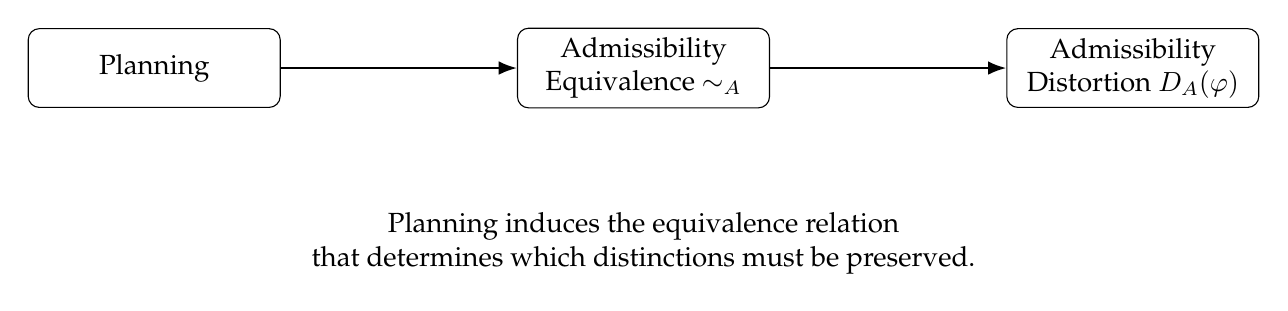
\begin{tikzpicture}[
  node distance=3cm,
  box/.style={draw,rounded corners,align=center,
              minimum width=3.2cm,minimum height=1cm}
]
\node[box] (planning) {Planning};
\node[box,right=of planning] (admissibility)
      {Admissibility\\Equivalence $\simA$};
\node[box,right=of admissibility] (distortion)
      {Admissibility\\Distortion $\DA$};
\draw[-Latex,thick] (planning) -- (admissibility);
\draw[-Latex,thick] (admissibility) -- (distortion);
\node[below=1.2cm of admissibility,align=center]
      {Planning induces the equivalence relation\\
       that determines which distinctions must be preserved.};
\end{tikzpicture}
\caption{Logical structure of the paper. Planning requirements induce the
admissibility equivalence relation~$\simA$, which in turn induces
admissibility distortion~$\DA$ as the canonical measure of
representational failure.}
\label{fig:core}
\end{figure}

\subsection{Universality and Minimality of Admissibility}

Proposition~\ref{prop:planning} establishes that $\simA$ is a necessary
condition for planning adequacy. A stronger result holds: $\simA$ is the
\emph{unique coarsest} equivalence relation that is safe for all
accessibility-based planning tasks simultaneously.

To state this precisely, restrict attention to the class $\mathfrak{T}_A$ of
\emph{accessibility tasks}: planning tasks whose cost functions depend only on
which future states are reachable, not on the particular trajectories by which
they are reached. This class includes reachability objectives, viability
problems, and any goal-conditioned task that asks whether a target is accessible
within horizon~$H$. For each $\mathcal{T} \in \mathfrak{T}_A$ with cost
function $c_{\mathcal{T}}$, define the \emph{task-preserving equivalence}
$\sim_{\mathcal{T}}$ by
\begin{equation}
  x_1 \sim_{\mathcal{T}} x_2
  \iff
  \text{the optimal policy from } x_1 \text{ equals that from } x_2
  \text{ under } c_{\mathcal{T}}.
\end{equation}

\begin{remark}
The restriction to $\mathfrak{T}_A$ is necessary. Tasks whose costs depend on
path length, energy expenditure, or trajectory risk may distinguish states with
identical reachability sets: two states may reach exactly the same futures at
different costs, inducing different optimal policies. Admissibility equivalence
is the maximal safe abstraction for accessibility structure. A richer notion of
admissibility incorporating path-cost structure would require extending
$\RHP(x)$ to an \emph{admissibility profile} $\mathcal{A}(x)$ that records
reachable states together with their access costs; we leave this extension for
future work.
\end{remark}

\begin{theorem}[Universality of Admissibility Equivalence]
\label{thm:universality}
\begin{equation}
  \simA \;=\; \bigcap_{\mathcal{T} \in \mathfrak{T}_A} \sim_{\mathcal{T}}.
\end{equation}
Two states are admissibility-equivalent if and only if no accessibility-based
planning task can distinguish them. Consequently, $\simA$ is the largest
equivalence relation contained in every task-preserving equivalence in
$\mathfrak{T}_A$:
\begin{equation}
  \text{if } {\sim} \subseteq {\sim_{\mathcal{T}}} \text{ for all }
  \mathcal{T} \in \mathfrak{T}_A,\text{ then } {\sim} \subseteq {\simA}.
\end{equation}
\end{theorem}

\begin{proof}
($\simA \subseteq \bigcap_{\mathcal{T}} \sim_{\mathcal{T}}$): If $x_1 \simA
x_2$, then $\RHP(x_1) = \RHP(x_2)$. For any accessibility task
$\mathcal{T} \in \mathfrak{T}_A$, the cost depends only on which future states
are reachable, and the reachable sets are identical, so optimal policies from
$x_1$ and $x_2$ must agree. Hence $x_1 \sim_{\mathcal{T}} x_2$ for all
$\mathcal{T} \in \mathfrak{T}_A$.

($\bigcap_{\mathcal{T}} \sim_{\mathcal{T}} \subseteq \simA$): Suppose
$\RHP(x_1) \neq \RHP(x_2)$. By Proposition~\ref{prop:planning}, there exists
an accessibility task $\mathcal{T}^* \in \mathfrak{T}_A$ for which the optimal
policies from $x_1$ and $x_2$ differ (assign zero cost to trajectories through
the distinguishing reachable state), so $x_1 \not\sim_{\mathcal{T}^*} x_2$,
and therefore $x_1 \notin \bigcap_{\mathcal{T}} \sim_{\mathcal{T}}$.

Maximality follows: any equivalence relation safe for all tasks in
$\mathfrak{T}_A$ is contained in their intersection, which equals $\simA$.
\end{proof}

Theorem~\ref{thm:universality} gives $\simA$ a representation-theoretic
character analogous to a sufficient statistic: it is the unique coarsest
representation that is safe for the entire class of accessibility-based
planning tasks. A representation may collapse any pair that $\simA$ identifies;
it may not safely collapse any other pair, because for every such pair there
exists an accessibility task that would be harmed. In this sense $\simA$ is the
maximally permissive safe quotient for accessibility-structured planning.

\subsection{Monotonicity of Admissibility Distortion}

Admissibility distortion behaves well with respect to the natural partial order
on quotient spaces. A coarser projection---one that collapses at least as many
distinctions---has distortion at least as large.

\begin{theorem}[Monotonicity]
\label{thm:monotone}
Let $\varphi_1, \varphi_2 : \mathcal{X} \to \mathcal{M}$ be projections with
induced equivalence relations ${\sim_{\varphi_1}} \subseteq {\sim_{\varphi_2}}$
(so $\varphi_2$ collapses at least every pair that $\varphi_1$ collapses).
Then
\begin{equation}
  D_A(\varphi_1) \leq D_A(\varphi_2).
\end{equation}
\end{theorem}

\begin{proof}
Every pair $(x_1, x_2)$ with $x_1 \sim_{\varphi_1} x_2$ also satisfies
$x_1 \sim_{\varphi_2} x_2$, since ${\sim_{\varphi_1}} \subseteq
{\sim_{\varphi_2}}$. Therefore the expectation defining $D_A(\varphi_2)$ sums
over a superset of the pairs summed over by $D_A(\varphi_1)$, and each term
is non-negative. Hence $D_A(\varphi_1) \leq D_A(\varphi_2)$.
\end{proof}

Theorem~\ref{thm:monotone} gives admissibility distortion the structure of an
order-preserving quantity on the lattice of quotient spaces ordered by coarseness.
The equivalence relations on $\mathcal{X}$ form a lattice under inclusion, with
the discrete relation (every pair distinct) at the bottom and the indiscrete
relation (all pairs collapsed) at the top. Admissibility distortion is monotone
increasing as one moves upward in this lattice toward coarser quotients.

The increase in distortion from $\varphi_1$ to $\varphi_2$ is not merely bounded;
it has an exact expression. Let $\mathcal{N} = {\sim_{\varphi_2}} \setminus
{\sim_{\varphi_1}}$ denote the set of newly collapsed pairs---pairs that
$\varphi_2$ identifies but $\varphi_1$ does not.

\begin{corollary}[Accounting Identity for Monotonicity]
\label{cor:accounting}
\begin{equation}
  D_A(\varphi_2) - D_A(\varphi_1)
  \;=\;
  \mathbb{E}\!\left[
    \mathbf{1}_{\mathcal{N}}(x_1, x_2)
    \cdot \Delta_A(x_1, x_2)
  \right].
\end{equation}
The increase in admissibility distortion is exactly the expected reachability
separation of the newly merged pairs.
\end{corollary}

\begin{proof}
$D_A(\varphi_2) = \mathbb{E}[\mathbf{1}_{\sim_{\varphi_2}} \cdot \Delta_A]
= \mathbb{E}[\mathbf{1}_{\sim_{\varphi_1}} \cdot \Delta_A]
+ \mathbb{E}[\mathbf{1}_{\mathcal{N}} \cdot \Delta_A]
= D_A(\varphi_1) + \mathbb{E}[\mathbf{1}_{\mathcal{N}} \cdot \Delta_A]$,
since ${\sim_{\varphi_2}} = {\sim_{\varphi_1}} \cup \mathcal{N}$ (disjoint union
by construction of $\mathcal{N}$).
\end{proof}

Corollary~\ref{cor:accounting} turns Theorem~\ref{thm:monotone} from an
inequality into an exact accounting identity. The additional distortion incurred
by moving from $\varphi_1$ to a coarser $\varphi_2$ is neither mysterious nor
an upper bound: it is literally the expected admissibility separation of the
pairs that the coarsening newly merges. A compression step that merges
mildly-separated pairs incurs small additional distortion; a step that merges
catastrophically-separated pairs---states that look statistically similar but
have radically different reachable futures---incurs large additional distortion.
This makes the cost of each compression decision explicit and in principle
auditable: one can evaluate whether a proposed coarsening is admissibility-safe
by examining the reachability separation of the pairs it would newly collapse.

The implications for compression are precise, and they are stronger than the
familiar observation that lossy compression discards information. The claim is
not that compression may occasionally drop something important. The claim is
that compression, understood as upward movement in the quotient lattice, is
formally ordered with respect to admissibility distortion: every step that
improves compression efficiency is a step that monotonically increases
admissibility risk. There exists a partial order on representations under which
better compressors are worse planners, not accidentally but by the structure of
the lattice. Compression does not merely risk admissibility failure; it is
structurally directed toward it. The pursuit of compression efficiency is, in
the quotient lattice, a directed walk toward higher distortion.

\subsection{Observational Sufficiency as a Characterisation}

Proposition~\ref{prop:coincidence} in Section~8 identifies the condition under
which prediction is admissibility-safe: ${\simO} \subseteq {\simA}$. A
characterisation theorem shows this condition has a precise interpretable meaning.

\begin{theorem}[Observational Sufficiency Characterisation]
\label{thm:obs_suff}
${\simO} \subseteq {\simA}$ if and only if every intervention-relevant variable
is observationally identifiable---that is, every variable whose value affects
$\RHP(x)$ is determined by the observation distribution $P(O_{t+1:t+k} \mid x)$.
\end{theorem}

\begin{proof}
($\Rightarrow$): Suppose ${\simO} \subseteq {\simA}$. If some variable $V$
affects reachability but is not determined by the observation distribution,
there exist states $x_1, x_2$ with $P(O \mid x_1) = P(O \mid x_2)$ (hence
$x_1 \simO x_2$) but with different values of $V$ and therefore different
reachability sets ($x_1 \not\simA x_2$). This contradicts ${\simO} \subseteq
{\simA}$.

($\Leftarrow$): Suppose every intervention-relevant variable is observationally
identifiable. If $x_1 \simO x_2$, then every variable that could affect
$\RHP(\cdot)$ takes the same value at $x_1$ and $x_2$ (since it is
observationally identifiable and the observation distributions coincide).
Therefore $\RHP(x_1) = \RHP(x_2)$, so $x_1 \simA x_2$.
\end{proof}

Theorem~\ref{thm:obs_suff} converts Proposition~\ref{prop:coincidence} from a
conditional statement into a characterisation: prediction is safe for planning
if and only if observation already contains admissibility. The condition is
precise and in principle testable. When it holds, predictive representations
are admissibility-preserving and $D_A(\varphi_P) = 0$. When it fails---when
any intervention-relevant variable is latent, unobservable, or
distribution-invariant under passive observation---the Observational--Interventional
Separation Theorem applies and $D_A(\varphi_P) > 0$ in general.

This result also clarifies the relationship between the admissibility framework
and domain-specific observability analyses in control theory. Classical
observability theory \citep{kalman1960general} asks whether the state can be
reconstructed from outputs; Theorem~\ref{thm:obs_suff} asks the more specific
question of whether the reachability-relevant part of the state can be recovered
from passive observations. The latter is a strictly weaker requirement than full
observability---it suffices that the intervention-relevant variables are
identifiable, not the entire state---but it is the requirement that matters for
planning adequacy.

\section{The Observational--Interventional Separation Theorem}

The admissibility distortion is positive whenever observational equivalence
fails to imply interventional equivalence. The paper's central theorem
establishes that this failure is not contingent but structural.

\begin{definition}[Observational Equivalence]
\label{def:obs}
States $x_1, x_2 \in \mathcal{X}$ are \emph{observationally equivalent},
$x_1 \simO x_2$, if for all $k \geq 1$,
\begin{equation}
  P\!\bigl(O_{t+1:t+k} \mid X_t = x_1\bigr)
  = P\!\bigl(O_{t+1:t+k} \mid X_t = x_2\bigr),
\end{equation}
where $O_{t+1:t+k}$ is the observation sequence under a fixed observational
(non-interventional) policy.
\end{definition}

\begin{definition}[Interventional Equivalence]
\label{def:int}
States $x_1, x_2 \in \mathcal{X}$ are \emph{interventionally equivalent},
written $x_1 \simI x_2$, if every admissible intervention yields identical
future accessibility: for all $\pi \in \Pi$ and all horizons $h \leq H$,
\begin{equation}
  \{y : x_1 \overset{\pi,h}{\rightsquigarrow} y\}
  = \{y : x_2 \overset{\pi,h}{\rightsquigarrow} y\}.
\end{equation}
\end{definition}

\begin{proposition}[Identification of Interventional and Admissibility Equivalence]
\label{prop:id}
${\simI} = {\simA}$.
\end{proposition}

\begin{proof}
By definition, $x_1 \simI x_2$ holds if and only if the reachable sets
from $x_1$ and $x_2$ coincide under every policy in $\Pi$ at every horizon
$h \leq H$. Taking $h = H$ and universally quantifying over $\pi$ yields
$\RHP(x_1) = \RHP(x_2)$, which is precisely $x_1 \simA x_2$. The reverse
direction is immediate since $\RHP(x) = \bigcup_{\pi \in \Pi}
\{y : x \overset{\pi,H}{\rightsquigarrow} y\}$.
\end{proof}

Proposition~\ref{prop:id} shows that the identification $\simI = \simA$ is a
theorem, not a definitional convenience. Interventional equivalence,
independently defined through identical accessibility under all policies, is
provably the same relation as admissibility equivalence derived from planning
requirements. These are categorically different objects at the definitional
level---observational equivalence is a statement about distributions over passive
sequences; interventional equivalence is a statement about geometry over
accessible futures---yet the coincidence $\simI = \simA$ is non-trivial and
underwrites the Separation Theorem's bite.


\begin{figure}[t]
\centering
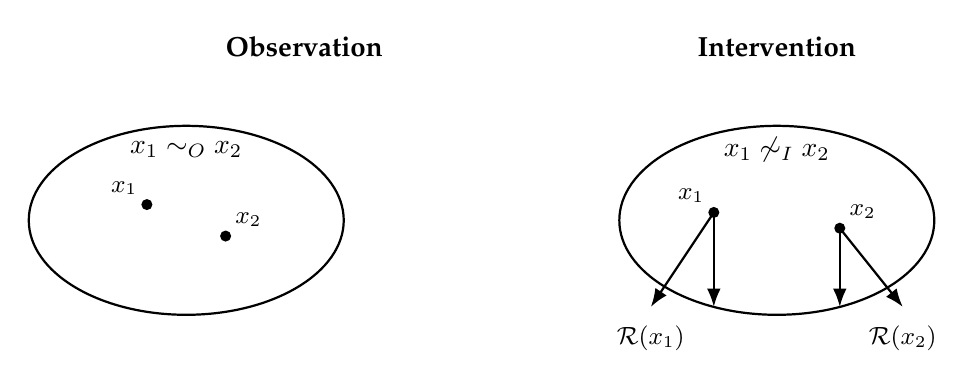
\begin{tikzpicture}[scale=1]
\node at (-3,2.2) {\textbf{Observation}};
\node at (3,2.2) {\textbf{Intervention}};

\draw[thick] (-4.5,0) ellipse (2.0 and 1.2);
\fill (-5.0,0.2) circle (2pt) node[above left]{\small$x_1$};
\fill (-4.0,-0.2) circle (2pt) node[above right]{\small$x_2$};
\node at (-4.5,0.9) {$x_1 \simO x_2$};

\draw[thick] (3,0) ellipse (2.0 and 1.2);
\fill (2.2,0.1) circle (2pt) node[above left]{\small$x_1$};
\fill (3.8,-0.1) circle (2pt) node[above right]{\small$x_2$};
\draw[-Latex,thick] (2.2,0.1) -- (1.4,-1.1);
\draw[-Latex,thick] (2.2,0.1) -- (2.2,-1.1);
\draw[-Latex,thick] (3.8,-0.1) -- (4.6,-1.1);
\draw[-Latex,thick] (3.8,-0.1) -- (3.8,-1.1);
\node at (1.4,-1.5) {\small$\mathcal{R}(x_1)$};
\node at (4.6,-1.5) {\small$\mathcal{R}(x_2)$};
\node at (3,0.9) {$x_1 \not\simI x_2$};
\end{tikzpicture}
\caption{Observational equivalence (left) compares distributions over
passive observation sequences; states $x_1$ and $x_2$ are grouped because
they produce identical observations. Interventional equivalence (right)
compares reachable futures; the same two states are separated because they
afford different reachability geometry. States may be observationally
indistinguishable yet interventionally inequivalent.}
\label{fig:oi}
\end{figure}

\begin{theorem}[Observational--Interventional Separation]
\label{thm:oi}
In general, $\simO \not\Rightarrow \simI$. There exist states
$x_1, x_2 \in \mathcal{X}$ that are observationally equivalent but
interventionally inequivalent.
\end{theorem}

\begin{proof}
It suffices to exhibit a class of systems in which the implication fails. Let
$x_1$ be a structurally intact load-bearing element and $x_2$ the same element
with an internal crack invisible to surface sensors. Under passive observation
over the operating range, $P(O_{t+1:t+k} \mid x_1) = P(O_{t+1:t+k} \mid x_2)$
for all relevant $k$, since the crack produces no observable surface deformation
under normal load---hence $x_1 \simO x_2$. Under a policy that applies
stress beyond the crack threshold, $x_2$ admits failure states not reachable
from $x_1$: $\RHP(x_1) \neq \RHP(x_2)$, so $x_1 \not\simI x_2$.

Reachability is not a local property of dynamics but a global property of
accessible futures: two states may have identical local transition structure
yet possess radically different reachability geometry, as the crack example
illustrates. More generally, any latent structural variable that determines reachability
without affecting current observation distributions---a hidden Markov state, an
unobservable causal parent, a dormant failure mode---produces the same pattern.
Such variables are ubiquitous in physical, biological, and engineered systems.

A minimal formal example makes the structure explicit. Let
$\mathcal{X} = \{s_0^0, s_0^1, s_{\text{safe}}, s_{\text{danger}}\}$, where
the superscript is a latent binary variable $L \in \{0,1\}$ not included in
the observation function. Define observations by $O(s_0^0) = O(s_0^1) = o_0$
(the two initial states are observationally identical), $O(s_{\text{safe}}) =
o_s$, $O(s_{\text{danger}}) = o_d$. Under a single action $a$: from $s_0^0$
action $a$ leads to $s_{\text{safe}}$; from $s_0^1$ action $a$ leads to
$s_{\text{danger}}$. Then $P(O_{t+1} \mid s_0^0) = P(O_{t+1} \mid s_0^1)$
for all passive observations (since both emit $o_0$), so $s_0^0 \simO s_0^1$.
But $\RHP(s_0^0) = \{s_{\text{safe}}\}$ while $\RHP(s_0^1) =
\{s_{\text{danger}}\}$, so $s_0^0 \not\simI s_0^1$. Any projection that
identifies $s_0^0$ with $s_0^1$ on the basis of their identical observations
is inadmissible, and a guardrail trained on observational data cannot separate
the safe from the dangerous initial condition.
\end{proof}

\begin{remark}[Structural Mismatch]
\label{rem:category}
The significance of Theorem~\ref{thm:oi} is not the existence of pathological
counterexamples but the fact that observational and interventional equivalence
are generated by operations of structurally different types. Observational equivalence is
generated by comparison of probability distributions over passive sequences:
$x_1 \simO x_2$ when $P(O \mid x_1) = P(O \mid x_2)$. Interventional
equivalence is generated by comparison of reachability geometry: $x_1 \simI x_2$
when $\RHP(x_1) = \RHP(x_2)$. These are different mathematical operations
producing different partition structures on $\mathcal{X}$: one compares
measures over observation sequences; the other compares subsets of the state
space under arbitrary interventions. The theorem identifies a structural mismatch
between equivalence-generating operations, not an empirical failure. This is why the gap cannot be
closed by improving the predictive model, collecting more data, or shifting
prediction from pixel space to latent space: none of those operations changes
the type of the equivalence relation being computed.
\end{remark}

The theorem connects to a central result in causal inference. Pearl's
do-calculus \citep{pearl2009causality} formalises precisely the gap between
observing and intervening: the distribution $P(Y \mid X = x)$ obtained by
passive observation differs in general from the distribution
$P(Y \mid \mathrm{do}(X = x))$ obtained by intervention. The present theorem
is the planning-theoretic analogue: the equivalence relation induced by
observation distributions differs in general from the equivalence relation
induced by intervention accessibility. A representation that respects
$\simO$ may fail to respect $\simI$, and a guardrail trained on observations
of a system may fail to detect dangerous states that are observationally
indistinguishable from safe ones.

The theorem also connects to the classical control-theoretic distinction between
system identification and reachability. A system identification procedure that
fits observational data yields a model accurate for prediction but potentially
inaccurate for control, because the identification experiments may not span the
relevant intervention space \citep{ljung1999system}. The identification-reachability
gap in control theory is the predecessor of the observational--interventional gap
formalised here.

The connection to \citet{gupta2025world} becomes precise at this point. Their
proof-understanding discussion invokes Poincar\'e's \citeyearpar{poincare1914}
distinction between verifying a proof step by step and understanding why the
steps are linked in a particular order. From the admissibility perspective,
this distinction maps onto the theorem directly. Verification corresponds to
checking local state transitions---the observational question of whether step
$s_{i+1}$ follows from $s_i$. Understanding corresponds to grasping why this
trajectory through proof space was selected from among the exponentially many
valid alternatives. That is a question about the reachability geometry of proof
space: which trajectories are accessible from the problem situation, and what
makes the chosen path salient. Verification is observational; understanding is
interventional. The structural mismatch identified in Remark~\ref{rem:category}
is why one does not imply the other.

\section{Three Corollaries: Prediction, Compression, and Safety}

Theorem~\ref{thm:oi} implies that both predictive and compressive projections
fail to guarantee admissibility in general, and that guardrail incompleteness
follows as an information-theoretic consequence.

\subsection{The Predictive Gap}

\begin{corollary}[Predictive Admissibility Gap]
\label{cor:pred}
Let $\varphi_P$ be a projection learned by minimising predictive loss, so that
$\varphi_P(x_1) = \varphi_P(x_2)$ whenever $x_1 \simO x_2$. Then
\begin{equation}
  D_A(\varphi_P) \not\equiv 0
\end{equation}
in general. Predictive sufficiency does not imply admissibility sufficiency.
\end{corollary}

\begin{proof}
By Theorem~\ref{thm:oi}, there exist states $x_1 \simO x_2$ with
$\RHP(x_1) \neq \RHP(x_2)$. A predictive projection identifies $x_1$ and
$x_2$, since they produce identical observation distributions. This
identification contributes positively to $D_A(\varphi_P)$.
\end{proof}

The JEPA planning loop presupposes that prediction-learned representations
correctly identify which futures are reachable, which distinctions are
decision-relevant, and which costs correctly measure proximity to the objective.
Corollary~\ref{cor:pred} establishes that none of these presuppositions are
established by predictive accuracy. A world model accurate in the predictive
sense may be inadmissible in the planning sense: it has collapsed distinctions
that separate accessible from inaccessible futures.

The point generalises beyond JEPA. Contrastive predictive coding
\citep{oord2018representation} learns representations by predicting future
observations in latent space; successor representations \citep{dayan1993improving}
encode discounted future state occupancy; general value functions
\citep{sutton2011horde} extend this to a large family of predictive knowledge
representations. All encode aspects of future observation structure. All remain
subject to the predictive gap because none directly optimise for preservation of
the reachability sets that Proposition~\ref{prop:planning} requires.

The anti-generative argument---that predicting in representation space is
superior to predicting in pixel space---is a local dispute within the shared
predictive assumption. Corollary~\ref{cor:pred} targets the assumption rather
than the dispute: moving prediction from one space to another does not change
the type of the equivalence relation being computed, and therefore does not close
the gap identified in Remark~\ref{rem:category}.

\subsection{The Compression Gap}

\begin{corollary}[Compression Admissibility Gap]
\label{cor:comp}
Let $\varphi_C$ be a projection learned by minimising description length.
Then ${\sim_{\varphi_C}} \not\subseteq {\simA}$ in general, and
\begin{equation}
  D_A(\varphi_C) \not\equiv 0.
\end{equation}
Compression sufficiency does not imply admissibility sufficiency.
\end{corollary}

\begin{proof}
A compressor succeeds by enlarging equivalence classes to reduce description
length. Admissibility permits identification only when $\RHP(x_1) = \RHP(x_2)$.
By Theorem~\ref{thm:oi}, there exist observationally equivalent pairs with
distinct reachability sets. A compressor operating on observation sequences
identifies such pairs, violating admissibility.
\end{proof}

The compression case warrants separate attention because the Schmidhuber tradition
\citep{schmidhuber1991possibility, schmidhuber2010formal} proposes compression
progress, not prediction accuracy, as the primary criterion for intelligence.
Corollary~\ref{cor:comp} shows that retreating from prediction to compression
does not escape the admissibility gap.

The quotient-space framing makes the structural reason transparent. Compression
objectives that are not constrained by admissibility reward enlarging
$\mathcal{X}/{\simC}$---making equivalence classes larger to reduce description
length. Admissibility constrains which enlargements are permitted---only those
that respect $\simA$. These pressures are opposed. A compression objective
unconstrained by admissibility is therefore not merely neutral with respect
to admissibility; it exerts active pressure toward admissibility-violating
identifications. This pressure is strongest precisely on rare, high-consequence
states that deviate from the training distribution---the distinctions that appear
as noise from the compressor's perspective and are therefore positive targets for
elimination, but which determine reachability at the boundaries where it matters
most. Compression objectives that incorporate admissibility-relevant distortion
measures---such as the task-weighted variant introduced in Section~8---can in
principle avoid this pressure, but unconstrained compression cannot.

The information bottleneck \citep{tishby1999information} provides the most
principled version of the compression account: a representation should retain
information about a target variable while discarding irrelevant variation. The
admissibility critique reframes the information bottleneck question. The relevant
question is not which information is retained about observed targets, but whether
the retained information preserves the reachability structure that planning
requires. A representation that maximally compresses toward an observed reward
signal may discard admissibility-relevant structure if that structure is not
correlated with the reward in the training distribution.

The \citeauthor{gupta2025world} argument about abstract-state inflation is
illuminating here. They observe that the world model framework can evade criticism
by adding increasingly abstract states, but that this manoeuvre undermines
falsifiability: if any cognitive phenomenon can be retrofitted as a state, the
framework becomes irrefutable. The admissibility framework avoids this problem
precisely because it does not ask what states a representation should contain
but whether the induced quotient $\mathcal{X}/{\sim_\varphi}$ is contained in
$\mathcal{X}/{\simA}$. This is a behavioural criterion defined over reachability
geometry, not an ontological criterion about representational content.
Admissibility distortion $\DA$ is in principle measurable; ``understanding''
is not. The distinction matters for whether a framework generates testable
predictions.

The failure mode identified in Corollary~\ref{cor:comp} is not merely epistemic.
When a compressive or predictive projection is deployed as a decision system, it
does not only fail to represent reachability structure---it actively alters that
structure. A hiring algorithm that collapses two applicants into the same latent
representation and rejects both narrows the reachable futures of those applicants
in ways the original training distribution did not reflect. The deployed projection
reshapes the state space it was trained to model. This creates a feedback dynamic
in which admissibility distortion compounds over deployment cycles: the projection
collapses a distinction, the resulting action enforces the collapse in the world,
and future training data reflects a state space in which the distinction has been
partially erased. \citet{veliz2024prophecy} identifies this as the self-fulfilling
structure of prediction; the admissibility framework supplies the formal criterion
for what is being destroyed. Admissibility distortion under a deployed projection
is not static. It accumulates.

\subsection{Guardrail Incompleteness}

\begin{corollary}[Safety--Admissibility Gap]
\label{cor:safety}
If $\DA > 0$ because the projection has identified states $x_s$ (safe) and
$x_d$ (dangerous) with $\varphi(x_s) = \varphi(x_d)$, then no guardrail
classifier operating on $\mathcal{M}$ alone can distinguish them.
\end{corollary}

This corollary concerns the claim that embedding a safety objective inside a
planning loop provides structural safety guarantees. The claim has surface
plausibility: a system architecturally required to pass every candidate action
through a constrained optimisation that includes a safety term cannot produce
an unsafe output without violating its own inference procedure. That is a genuine
advantage over unconstrained generation.

The hidden assumption is that the projection preserves every distinction relevant
to whether an action is dangerous. When this assumption fails---when $\DA > 0$
in the relevant region of state space---the advantage evaporates. The safety
problem has been relocated: from aligning a generative model's output distribution
to guaranteeing that a projection head correctly identifies every dangerous state
from a small number of examples, in a latent space organised around a predictive
objective that does not treat dangerousness as a primary criterion.

The corollary can be strengthened first by a constructive argument, and then to
a general information-theoretic theorem. The constructive argument requires no
measure theory. Suppose $\varphi(x_s) = \varphi(x_d) = z$ for some safe state
$x_s$ and dangerous state $x_d$, with $A(x_s) = 0$ and $A(x_d) = 1$. Any
classifier $G : \mathcal{M} \to \{0,1\}$ operating on the projection receives
the same input $z$ from both states. Since $G$ is a function, $G(z) =
G(\varphi(x_s)) = G(\varphi(x_d))$. Therefore $G$ must output the same label
for both, and one of the two states is necessarily misclassified. No classifier,
of any architecture or complexity, can separate $x_s$ from $x_d$ once $\varphi$
has identified them. The failure is a consequence of the projection, not of any
property of the classifier. The general form is given first; the impossibility result follows as a special case.

\begin{theorem}[Irrecoverable Quotient Collapse]
\label{thm:guardrail}
Let $A$ be a random variable indicating admissibility status. Let
$\varphi : \mathcal{X} \to \mathcal{M}$ be a projection. Then for every
downstream transformation $G : \mathcal{M} \to \{0,1\}$,
\begin{equation}
  I\!\left(A;\, G(\varphi(X))\right)
  \leq I\!\left(A;\, \varphi(X)\right).
\end{equation}
In particular, if $I(A;\, \varphi(X)) = 0$, then $I(A;\, G(\varphi(X))) = 0$:
no downstream computation recovers admissibility information absent from the
projection.
\end{theorem}

\begin{proof}
The full Markov chain is $A \to X \to \varphi(X) \to G(\varphi(X))$: $A$
causally determines $X$; the projection $\varphi$ is a deterministic function
of $X$; and $G$ is a deterministic function of $\varphi(X)$. Each link in
the chain satisfies the Markov property. The data-processing inequality
\citep{cover2006elements} states that mutual information cannot increase along
a Markov chain, so
\begin{equation}
  I\!\left(A;\, G(\varphi(X))\right)
  \leq I\!\left(A;\, \varphi(X)\right).
\end{equation}
The special case follows immediately: if $I(A;\, \varphi(X)) = 0$, then
$I(A;\, G(\varphi(X))) \leq 0$, and since mutual information is non-negative,
equality holds.
\end{proof}


\begin{figure}[t]
\centering
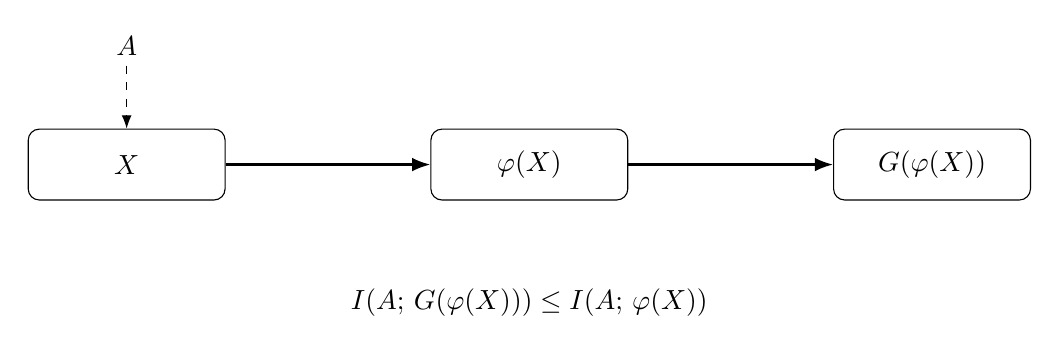
\begin{tikzpicture}[
  node distance=2.6cm,
  box/.style={draw,rounded corners,align=center,
              minimum width=2.5cm,minimum height=0.9cm}
]
\node[box] (x)   {$X$};
\node[box,right=of x]   (phi) {$\varphi(X)$};
\node[box,right=of phi] (g)   {$G(\varphi(X))$};
\draw[-Latex,thick] (x)   -- (phi);
\draw[-Latex,thick] (phi) -- (g);
\node[above=0.8cm of x] (a) {$A$};
\draw[-Latex,dashed] (a) -- (x);
\node[below=1.0cm of phi,align=center]
      {$I(A;\,G(\varphi(X))) \leq I(A;\,\varphi(X))$};
\end{tikzpicture}
\caption{Irrecoverable quotient collapse (Theorem~\ref{thm:guardrail}).
The admissibility variable~$A$ determines whether a state is safe or
dangerous. After projection through~$\varphi$, the mutual information
between~$A$ and any downstream classifier~$G$ is bounded above by
$I(A;\,\varphi(X))$. Distinctions destroyed by the projection cannot
be recovered by any downstream computation.}
\label{fig:dpi}
\end{figure}

The general bound in Theorem~\ref{thm:guardrail} is the more useful result in
practice: real projections are unlikely to destroy all admissibility information,
but they may reduce it substantially. Any downstream classifier---whether a
linear safety head, a learned guardrail, or a constrained optimiser---can do no
better than the admissibility information the projection retains. The upper bound
$I(A;\, \varphi(X))$ is therefore a hard ceiling on the performance of any
downstream safety mechanism, regardless of the mechanism's complexity.

The impossibility corollary identifies the boundary case: when the projection
collapses a distinction that is completely admissibility-relevant, no downstream
computation can recover it. The failure precedes optimisation entirely. It is
not a failure of the optimiser; it is a failure of the quotient. This formulation
differs from the dominant class of alignment critiques, which argue that an
optimiser may exploit loopholes in a safety specification. The present result
operates at a different level: if safety-relevant information is absent from the
projection, there is no representation of the distinction to be exploited or
circumvented.

Popper's problem-situation account \citep{popper1979objective}, as discussed by
\citet{gupta2025world}, provides a suggestive parallel at the level of
explanatory understanding. Popper argues that understanding a physical theory
requires grasping the problem situation---the theoretical landscape and
explanatory gaps that motivated the theory. This can be reinterpreted in
admissibility terms: the problem situation acts as a constraint structure over
the space of possible theoretical moves, partitioning them into those that address
the identified problems and those that do not. A representation that fails to
encode the problem situation cannot identify which theoretical moves are
explanatorily accessible. The guardrail incompleteness theorem is the formal
analogue: a projection that destroys the relevant constraint structure cannot
support any downstream classifier that depends on it.

The mutual-information bound of Theorem~\ref{thm:guardrail} can be translated
into a classification error floor that makes the engineering implication concrete.

\begin{corollary}[Bayes-Risk Floor]
\label{cor:bayes}
Let $A \in \{0,1\}$ be the admissibility indicator (safe/dangerous), with
prior $p = P(A=1)$. Let $\varphi : \mathcal{X} \to \mathcal{M}$ be a
projection, and let $G : \mathcal{M} \to \{0,1\}$ be any classifier. Define
the Bayes error of any classifier on $\varphi(X)$ as
$\varepsilon^* = \min_G P(G(\varphi(X)) \neq A)$.
By Fano's inequality \citep{cover2006elements},
\begin{equation}
  \varepsilon^* \;\geq\; \frac{H(A) - I(A;\,\varphi(X)) - 1}{\log 2},
\end{equation}
where $H(A) = -p\log p - (1-p)\log(1-p)$ is the binary entropy of $A$.
Consequently, if $I(A;\,\varphi(X)) < H(A) - 1$ (in nats), no binary
classifier operating on $\mathcal{M}$ can achieve Bayes error below
$\varepsilon^*$, regardless of the classifier's complexity.
\end{corollary}

\begin{proof}
Fano's inequality states that for any Markov chain $A \to Z$ and any estimator
$\hat{A}(Z)$, $P(\hat{A} \neq A) \geq (H(A|Z) - 1)/\log|\mathcal{A}|$. With
$Z = \varphi(X)$, $|\mathcal{A}| = 2$, and $H(A \mid \varphi(X)) = H(A) -
I(A;\,\varphi(X))$, the bound follows directly. By
Theorem~\ref{thm:guardrail}, $I(A;\,G(\varphi(X))) \leq I(A;\,\varphi(X))$
for any $G$, so the same floor applies to all downstream classifiers.
\end{proof}

Corollary~\ref{cor:bayes} converts the abstract mutual-information ceiling into
a concrete, calculable lower bound on misclassification rate. The practical
consequence is that engineering effort spent on classifier architecture or
training procedures cannot improve on $\varepsilon^*$: the error floor is set by
the projection, not the classifier. In high-stakes domains where the prior is
balanced ($p \approx 0.5$, $H(A) \approx 1$ nat) and admissibility information in
the projection is low, $\varepsilon^*$ approaches $0.5$---random guessing. A
safety architect who does not know $I(A;\,\varphi(X))$ does not know the ceiling
on their classifier's performance; a safety architect who does know it can identify
whether the problem is the classifier or the representation. This is the
operational use of the bound: not as a training signal, but as a diagnostic that
identifies whether safety failure is attributable to classifier inadequacy or
to representational inadmissibility.

\section{Collapse as Quotient Selection}

The technical literature treats representational collapse as a pathology and
engineers various anti-collapse mechanisms: exponential moving average target
encoders, information maximisation objectives, contrastive terms. These mechanisms
prevent the trivial collapse in which all inputs map to a single representation.
They do not prevent the more subtle and consequential collapse described by
Theorem~\ref{thm:oi}.

Every abstraction is a quotient map $q : \mathcal{X} \to \mathcal{X}/{\sim}$.
The anti-trivial-collapse mechanisms constrain the global distribution of the
induced equivalence classes without constraining which states are identified.
Information maximisation objectives such as VICReg require that representation
components be approximately independent and that the empirical distribution
approximate an isotropic Gaussian. This ensures that the representation space
is broadly used---that $\mathcal{X}/{\sim_\varphi}$ has many distinct
elements---but does not constrain whether the boundaries of those elements
respect $\simA$.


\begin{figure}[t]
\centering
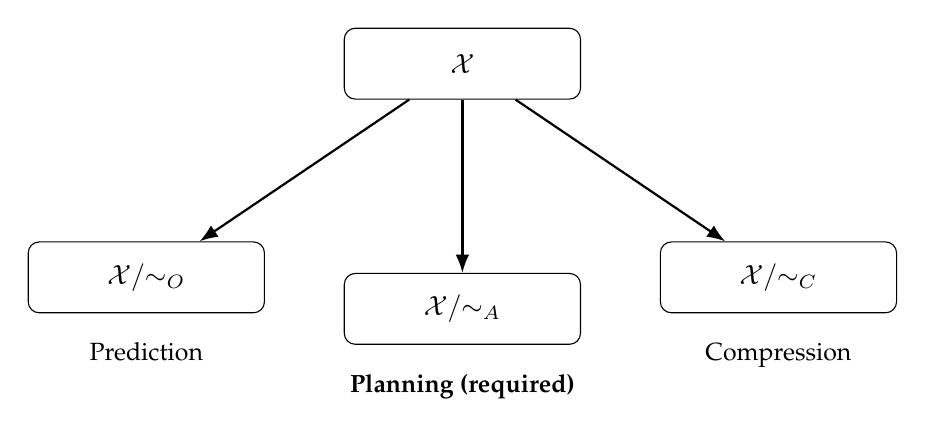
\begin{tikzpicture}[
  node distance=2.0cm,
  box/.style={draw,rounded corners,align=center,
              minimum width=3cm,minimum height=0.9cm}
]
\node[box] (world) {$\mathcal{X}$};
\node[box,below left=1.8cm and 1.0cm of world]  (obs)  {$\mathcal{X}/{\simO}$};
\node[box,below=2.2cm of world]                 (adm)  {$\mathcal{X}/{\simA}$};
\node[box,below right=1.8cm and 1.0cm of world] (comp) {$\mathcal{X}/{\simC}$};
\draw[-Latex,thick] (world) -- (obs);
\draw[-Latex,thick] (world) -- (adm);
\draw[-Latex,thick] (world) -- (comp);
\node[below=0.25cm of obs]  {\small Prediction};
\node[below=0.25cm of adm]  {\small\textbf{Planning (required)}};
\node[below=0.25cm of comp] {\small Compression};
\end{tikzpicture}
\caption{Representation learning as quotient selection
(Proposition~\ref{prop:quotient}). Each learning objective induces a
different equivalence relation on the state space~$\mathcal{X}$ and thereby
proposes a different quotient. The admissibility quotient
$\mathcal{X}/{\simA}$ is the quotient that planning requires; predictive
and compressive quotients are evaluated by how well they approximate it.}
\label{fig:quotients}
\end{figure}

Viewed this way, the dispute between JEPA, latent diffusion, transformer-based
world models, bisimulation learning, predictive state representations, and
compression-based intelligence is a dispute about quotient selection. Each
approach proposes a different equivalence relation: $\simO$ for predictive
approaches, $\simC$ for compressive approaches, bisimulation equivalence for
bisimulation-based approaches. The admissibility question is in each case the
same: does ${\sim_\varphi} \subseteq {\simA}$? The renormalisation-group
perspective in physics \citep{wilson1975renormalization} asks a closely related
question: which distinctions survive coarse-graining? The admissibility question
inverts this: which distinctions must not be coarse-grained? The answer
determines which quotients are compatible with planning.

\begin{proposition}[Representation Learning as Quotient Selection]
\label{prop:quotient}
Every representation-learning method is, at the level of its induced
equivalence classes, a proposal for a quotient of the state space
$\mathcal{X}/{\sim_\varphi}$. Methods differ not in whether they select a
quotient but in which quotient they select. Predictive methods select
$\mathcal{X}/{\simO}$; compressive methods select $\mathcal{X}/{\simC}$;
bisimulation-based methods select $\mathcal{X}/{\sim_{\text{bis}}}$. The
admissibility question is, in every case, whether the selected quotient is
contained in $\mathcal{X}/{\simA}$:
\begin{equation}
  {\sim_\varphi} \subseteq {\simA}.
\end{equation}
The choice of representation is therefore not primarily a choice of architecture
or objective function. It is a choice of equivalence relation over reality.
\end{proposition}

\section{Admissibility as Prior Condition}

The foregoing critique might be resisted as follows. Every framework assumes
something; the admissibility framework assumes reachability structure while the
predictive framework assumes predictive structure. Why should one be privileged?

The objection would be correct if admissibility were simply another objective.
Proposition~\ref{prop:planning} establishes that it is not. Admissibility is
the condition derived from what planning requires, not a competing desideratum.
Consider the full range of goals a planning architecture might pursue: prediction,
compression, control, reward, and safety. Each requires the system to distinguish
states with different future trajectories. Prediction asks which future occurs.
Compression asks which structure can be simplified. Control asks how to reach a
desired future. Reward asks which futures are preferred. Safety asks which
futures are forbidden. Every question presupposes that distinct futures can be
distinguished and that some are accessible while others are not. That
presupposition is what admissibility formalises, and it is derived from the
structure of planning rather than assumed as a primitive.

The relationship between admissibility and classical model-predictive control
\citep{mayne2000model, garcia1989model} clarifies the scope of the claim.
Classical MPC assumes that state variables have already been correctly chosen,
that the representation is a sufficient statistic for future evolution under
admissible policies. The hard problem in MPC is state estimation and model
identification---prior problems treated before optimisation begins. The genuinely
novel claim in JEPA-based world models is that self-supervised latent
representations learned by predicting masked video constitute such sufficient
statistics. Corollary~\ref{cor:pred} establishes that this claim is unproven
and that the criterion by which it could be evaluated is precisely $\DA$.

Admissibility also clarifies the relationship to Gibson's ecological approach
\citep{gibson1979ecological}. Gibson argued that perception is organised around
affordances---what an environment permits---rather than around object identity.
The admissibility framework makes a structurally similar move in representation
learning: a representation is adequate not insofar as it accurately encodes
object properties but insofar as it preserves the distinctions that determine
what actions the current state affords. Both afford-based and admissibility-based
accounts shift the representational question from \emph{what is this?} to
\emph{what can I do from here?}

It is important to note what the admissibility framework does and does not claim.
The paper does not assert that planning, understanding, and safe action are
identical phenomena. It claims only that all three require preservation of
distinctions that alter reachable futures. Admissibility is proposed as a
common necessary condition, not a sufficient characterisation of any of these
phenomena. A system with low admissibility distortion may still fail at
understanding for reasons that the present framework does not address. The claim
is the weaker and more defensible one: that inadmissibility is a sufficient
condition for failure at planning, a necessary condition for adequate planning,
and a plausibly necessary condition for the kinds of understanding that Gupta
and Pruthi describe---but not a complete account of any of them.

\section{Toward Admissibility-Preserving Representation Learning}

The critique identifies a missing criterion and thereby defines a research
agenda. Representation learning currently lacks methods for measuring, bounding,
or regularising $\DA$. Several concrete directions follow from the definition.

\subsection{Relational Form and Metric Independence}

Before turning to estimation, it is important to clarify that admissibility
distortion is not inherently dependent on explicit simulation of reachability sets.
The reachability-set formulation in Definition~\ref{def:distortion} is the direct
semantic definition, but the same object can be expressed relationally without
presupposing a simulator.

The primitive failure is the existence of a pair with $x_1 \sim_\varphi x_2$ and
$x_1 \not\simA x_2$. Admissibility distortion measures the extent of such
violations:
\begin{equation}
  \DA
  = \mathbb{E}_{x_1,x_2}\!\left[
      \mathbf{1}_{x_1 \sim_\varphi x_2}
      \cdot \mathbf{1}_{x_1 \not\simA x_2}
      \cdot \delta_A(x_1,x_2)
    \right],
\end{equation}
where $\delta_A$ is any non-negative severity functional satisfying
$\delta_A(x_1,x_2) = 0 \iff x_1 \simA x_2$. The Hausdorff distance between
reachable sets is one realisation of $\delta_A$, not the unique choice.
The theory requires only that the severity functional vanish exactly on
admissibility-equivalent pairs. This separates the formal criterion from any
particular estimation method.

Equivalently, $\varphi$ is admissible if and only if it factors through the
admissibility quotient: there exists $\bar{\varphi}$ such that the diagram
\begin{equation}
  \mathcal{X} \xrightarrow{\;\varphi\;} \mathcal{M}
  \quad\text{factors as}\quad
  \mathcal{X} \xrightarrow{q_A} \mathcal{X}/{\simA} \xrightarrow{\;\bar{\varphi}\;} \mathcal{M},
\end{equation}
where $q_A$ is the canonical quotient map. Admissibility distortion is zero if
and only if such a factorisation exists. In this form, admissibility failure is
a quotient-factorisation failure, and the identification of $\DA$ with specific
metrics is a matter of estimation rather than definition.

The identification of $\DA$ as a formal quantity logically precedes the
development of efficient estimators for it. Entropy was conceptually central
before practical entropy estimators existed; Kolmogorov complexity is important
despite being incomputable; Wasserstein distance became computationally practical
long after its mathematical significance was established. A criterion does not
need an immediate estimator to establish its role as the right target. Developing
practical estimators for $\DA$---through bisimulation bounds, forward rollout,
reachability analysis \citep{tomlin2003computational}, or task-specific
approximations---is a concrete and tractable research program subsequent to
identifying the quantity.

It is important to be explicit about what $\DA$ currently is and what it is not. 
The contribution of this paper is not an estimator for admissibility distortion.
It is the identification of admissibility distortion as the quantity whose
estimation future work must address. $\DA$ is at present a foundational diagnostic
criterion rather than a deployed engineering metric. Lower bounds via bisimulation
and trajectory sampling (Propositions~\ref{prop:bisim_bound}
and~\ref{prop:lower_bound}) can reveal witnessed violations and identify
high-distortion regions, but absence of detected violation is not a certificate of
admissibility: the bounds are conservative, and safety-critical regions are
precisely those where exploration is most restricted. A representation that satisfies
current estimable lower bounds may still have $\DA > 0$ in unobserved regions of
the state space. The research agenda is therefore not merely to compute $\DA$ but
to develop estimators that are eventually tight in expectation and certificates that
are eventually sound. This is the work the criterion makes possible; it is not work
the paper claims to have completed. The paper's real claim is that current
representation learning is optimising the wrong target, and that the right target
is $\DA$. Whether $\DA$ becomes a practical loss function depends on progress in
reachability estimation, offline dynamics modelling, and adversarial state-space
exploration---problems that the admissibility framework helps organise but does
not solve.

The asymmetry between positive and negative evidence from trajectory sampling
is worth formalising.

\begin{proposition}[Asymmetry of Lower-Bound Evidence]
\label{prop:asymmetry}
Let $\Pi_{\mathrm{test}} \subseteq \Pi$ be any test policy set. Then
$\hat{D}_A(\varphi; \Pi_{\mathrm{test}}, H) \leq \DA$ (Proposition~\ref{prop:lower_bound}).
Consequently:
\begin{enumerate}
  \item If $\hat{D}_A(\varphi; \Pi_{\mathrm{test}}, H) > 0$, then $\DA > 0$:
    a positive estimate \emph{proves} that admissibility distortion exists.
  \item If $\hat{D}_A(\varphi; \Pi_{\mathrm{test}}, H) = 0$, this does not
    imply $\DA = 0$: a zero estimate proves only that \emph{the sampled policies
    failed to witness a violation}, not that no violation exists.
\end{enumerate}
\end{proposition}

\begin{proof}
Part 1 follows immediately from the lower-bound relation: $\hat{D}_A > 0$ implies
$\DA \geq \hat{D}_A > 0$. Part 2 follows from the set-inclusion
$\hat{\mathcal{R}}^{\Pi_{\mathrm{test}}, H}(x) \subseteq \RHP(x)$: if
$\Pi_{\mathrm{test}}$ fails to reach the states that witness the reachability
divergence, the empirical reachability sets may agree even when the true sets
differ.
\end{proof}

The asymmetry is the same as in model checking, adversarial testing, and
fuzzing: finding a counterexample is a definitive result; failing to find one
is not a proof of correctness. It implies that trajectory-sampling audits are
one-sided diagnostic tools. High-distortion pairs, when found, are genuine
failures and can be used to improve or reject the projection. Zero estimated
distortion under a test policy set is an absence of witnessed evidence, not a
safety certificate. The practical consequence is that the value of an audit
increases with the diversity and adversarial coverage of $\Pi_{\mathrm{test}}$,
since wider coverage shrinks the gap between $\hat{D}_A$ and $\DA$. Constructing
$\Pi_{\mathrm{test}}$ to maximise this coverage---through policy diversity
objectives, reachability-guided exploration, or learned adversarial policies---is
the operational problem that sits between the criterion and its engineering use.

\subsection{Task-Weighted Distortion}

Not every reachability difference has equal planning significance. A projection
that collapses two states with slightly different reachable sets in a dynamically
irrelevant region does not incur the same failure as one that collapses a safe
state with a dangerous one. The natural refinement is a task-weighted admissibility
distortion:
\begin{equation}
  D_A^w(\varphi)
  = \mathbb{E}_{x_1,x_2}\!\left[
      \mathbf{1}_{\varphi(x_1)=\varphi(x_2)}
      \cdot w(x_1,x_2)
      \cdot d\!\left(\RHP(x_1),\RHP(x_2)\right)
    \right],
\end{equation}
where $w(x_1,x_2) \geq 0$ weights reachability differences by their relevance
to the task, safety envelope, or constraint boundary. The unweighted distortion
$\DA$ asks whether the projection is admissible in the strict sense; the weighted
distortion $D_A^w$ asks where inadmissibility matters most.

This formulation also sharpens the argument against compression. Rare states have
low probability under the training distribution but often high weight under the
safety or task distribution. A compressor is rewarded for eliminating statistically
rare distinctions; admissibility penalises the elimination of reachability-critical
distinctions. Compression acts as an active pressure against safety by treating
outliers as noise---where ``outliers'' from the compressor's perspective may be
precisely the boundary conditions, tail risks, and irreversible transitions that
planning most needs to distinguish. The conflict is not accidental. It arises
because the probability measure used for compression and the importance measure
used for planning need not agree, and in safety-critical domains they are
systematically opposed.

\subsection{Horizon Hierarchy and Admissibility Depth}

Admissibility equivalence is parameterised by the horizon $H$ and policy
class $\Pi$: $\simA$ is really $\sim_A^{(\Pi,H)}$. This parameterisation
implies a natural hierarchy. Longer planning horizons split equivalence classes
that shorter horizons leave merged:
\begin{equation}
  \sim_A^{(\Pi,H=1)}
  \;\supseteq\;
  \sim_A^{(\Pi,H=10)}
  \;\supseteq\;
  \cdots
  \;\supseteq\;
  \sim_A^{(\Pi,H=\infty)}.
\end{equation}
Two states may be admissibility-equivalent for planning over one step yet
separable for planning over ten steps. This suggests a natural measure of
how fine-grained a distinction is:

\begin{definition}[Admissibility Depth]
\label{def:depth}
The \emph{admissibility depth} of a pair $(x_1, x_2)$ is
\begin{equation}
  d_A(x_1, x_2)
  = \min\bigl\{H \in \mathbb{N}
    : x_1 \not\sim_A^{(\Pi,H)} x_2\bigr\},
\end{equation}
with $d_A(x_1, x_2) = \infty$ if $x_1 \simA x_2$ for all $H$.
\end{definition}

A large admissibility depth means two states are nearly equivalent for
short-horizon planning but diverge at longer horizons. This connects directly
to the verification/understanding distinction from Section~4: verification of
local proof steps is a small-$H$ problem, while understanding the global
trajectory through proof space requires large $H$. A representation adequate
for one-step prediction may be catastrophically inadmissible for strategic
planning.

\subsection{Structural and Operational Distortion}

Definition~\ref{def:distortion} computes $\DA$ as an expectation over pairs
drawn from the state distribution induced by the agent's current policy. This
yields the \emph{operational distortion} $D_A^\pi(\varphi)$: the distortion
on states the agent actually encounters. It is the quantity that matters for
average-case planning performance.

A complementary quantity is the \emph{structural distortion}:
\begin{equation}
  D_A^{\text{struct}}(\varphi)
  = \sup_{x_1, x_2 \in \mathcal{X}}
    \mathbf{1}_{\varphi(x_1)=\varphi(x_2)}
    \cdot d\!\left(\RHP(x_1), \RHP(x_2)\right),
\end{equation}
measuring the worst-case admissibility violation over the entire state space,
regardless of visit frequency. The two quantities can diverge dramatically.
A projection can have $D_A^\pi(\varphi) \approx 0$ under a conservative policy
while $D_A^{\text{struct}}(\varphi) \gg 0$ in rarely visited regions. This
distinction is critical for safety: catastrophic failures characteristically
occur in low-frequency, high-consequence regions of state space---the same
regions that operational distortion underweights. A safety certificate based
on $D_A^\pi$ may therefore provide a false assurance about structural
admissibility. The task-weighted distortion $D_A^w(\varphi)$ of
the task-weighted distortion $D_A^w$ introduced above interpolates between these extremes when $w$ assigns high weight
to safety-critical regions regardless of their visit frequency.

\subsection{The Coincidence Regime and Limits of the Separation}

The Observational--Interventional Separation Theorem establishes that
$\simO \not\Rightarrow \simI$ in general. It does not assert that observational
and interventional equivalence always diverge. The following proposition clarifies
the conditions under which predictive representations can be admissibility-preserving.

\begin{proposition}[Coincidence Conditions]
\label{prop:coincidence}
Suppose that ${\simO} \subseteq {\simA}$---that every observationally equivalent
pair is also admissibility-equivalent. Then a predictive projection $\varphi_P$
satisfying $\varphi_P(x_1) = \varphi_P(x_2)$ whenever $x_1 \simO x_2$ is
admissible, and $D_A(\varphi_P) = 0$.
\end{proposition}

\begin{proof}
If ${\simO} \subseteq {\simA}$, then every pair collapsed by $\varphi_P$ is an
admissibility-equivalent pair, so no collapsed pair contributes positively to
$D_A(\varphi_P)$, hence $D_A(\varphi_P) = 0$.
\end{proof}

The condition ${\simO} \subseteq {\simA}$ is an additional structural property
of the system and the observational process, not a consequence of predictive
training. It holds when the observational policy exposes every intervention-relevant
variable---when no hidden structural variable determines reachability without
affecting observation distributions. In such systems, predictive representations
can be safe for planning relative to $(\Pi, H)$. The framework does not deny
that prediction can work; it specifies the exact condition under which prediction
is permitted to work. The condition is ${\simO} \subseteq {\simA}$. Verifying
this condition is an independent problem that predictive training does not address.

\emph{Estimation and connections.} Developing practical estimators for $\DA$ is
a concrete research problem. Bisimulation metrics \citep{ferns2004metrics} provide
lower bounds on reachability divergence. Approximate reachability analysis
\citep{tomlin2003computational} provides formal bounds in continuous systems.

\emph{Regularisation.} Once estimable, $\DA$ can be incorporated as a
regularisation term in the representation learning objective. An encoder trained
to minimise predictive loss plus admissibility distortion would face an explicit
tension: collapsing pairs reduces prediction error but increases distortion if
the pair is admissibility-inequivalent. This tension would make the
admissibility cost of each representational choice visible rather than hidden.

\emph{Projection auditing.} Existing representations can be audited post hoc
without retraining. Given a trained encoder and a forward model, pairs of states
that the encoder collapses can be sampled and their reachability sets compared.
High-distortion pairs identify failure modes: the collapsing of distinctions that
planning requires to be preserved. Theorem~\ref{thm:guardrail} provides a formal
motivation for this practice: the quantity $I(A;\, \varphi(X))$ places a hard
ceiling on downstream safety classifier performance, and auditing estimates this
ceiling directly.

\emph{Future-cone metrics.} The metric $d$ in Definition~\ref{def:distortion}
admits multiple implementations. Hausdorff distance between reachable sets is
one choice; asymmetric set-inclusion losses provide another; measure-theoretic
distances over reachable distributions and task-weighted metrics emphasising
reachability divergence in high-value regions provide others. Developing the
space of admissibility metrics connects to optimal transport and metric geometry.

\begin{proposition}[Bisimulation Lower Bound]
\label{prop:bisim_bound}
Let $D_{\text{bisim}}(\varphi)$ denote the bisimulation distortion of
$\varphi$---the expected difference in value functions between collapsed
states under the bisimulation metric \citep{ferns2004metrics}. Under
reward functions that depend only on reachability structure,
\begin{equation}
  D_{\text{bisim}}(\varphi) \;\leq\; C \cdot \DA
\end{equation}
for a constant $C$ depending on the reward scale and discount factor. In
particular, $\DA = 0$ implies $D_{\text{bisim}}(\varphi) = 0$: admissibility
subsumes bisimulation for accessibility-structured rewards.
\end{proposition}

\begin{proof}[Proof sketch]
If two states are admissibility-equivalent ($\RHP(x_1) = \RHP(x_2)$), they
reach the same futures and therefore have the same optimal value under any
accessibility-structured reward. Hence their bisimulation distance is zero.
The bound in the non-zero case follows from the Lipschitz continuity of value
functions with respect to reachability divergence under standard assumptions
on the reward and discount; the constant $C$ absorbs the reward scale and
$1/(1-\gamma)$ from the geometric series.
\end{proof}

Proposition~\ref{prop:bisim_bound} provides a computable surrogate:
bisimulation metrics, which are implemented in several representation
learning systems, serve as lower bounds on admissibility distortion. A
representation with high bisimulation distortion necessarily has high
admissibility distortion; a representation with low bisimulation distortion
may still have high admissibility distortion in regions the bisimulation
metric does not resolve. This relationship suggests a practical estimation
strategy: use bisimulation metrics as a conservative lower bound, and
supplement with targeted reachability probes in high-stakes regions.

\begin{remark}[Stochastic Extension]
\label{rem:stochastic}
For clarity of exposition, the paper treats the deterministic case where
$\RHP(x)$ is a set of reachable states. The extension to stochastic dynamics
is conceptually straightforward. The reachability set $\RHP(x)$ is replaced
by a distribution over future trajectories $P(\cdot \mid x, \pi, H)$, and
admissibility equivalence becomes equality of these distributions for all
$\pi \in \Pi$. The set-distance metric $d$ is replaced by a divergence
between distributions---Wasserstein distance or KL divergence are natural
choices. The Observational--Interventional Separation Theorem remains
unchanged in structure: passive observation yields a distribution over
observation sequences, while intervention yields a distribution over reachable
trajectory distributions; these are different mathematical objects for the
same reasons as in the deterministic case. The admissibility distortion
$\DA$ becomes a measure of divergence between collapsed reachable
distributions, and the data-processing inequality in
Theorem~\ref{thm:guardrail} applies without modification.
\end{remark}

\emph{Structural connections.} The Li--Walsh--Littman \citeyearpar{li2006towards}
abstraction hierarchy identifies which collapse relations are compatible with
optimal policy preservation; admissibility extends the question beyond
value-function equivalence to reachability-set equivalence. The information
bottleneck \citep{tishby1999information} minimises $I(X; Z)$ subject to a
constraint on $I(Z; Y)$; substituting the admissibility signal for $Y$ yields
an admissibility-constrained bottleneck, which would enforce that the retained
information includes the reachability-relevant distinctions planning requires.
Bisimulation metrics \citep{ferns2004metrics} provide a continuous relaxation
of equivalence that could be extended to the reachability-set setting, yielding
approximate admissibility conditions suitable for continuous domains.

The broader shift the admissibility framework enables is a reorientation of what
representation learning for planning is understood to optimise. The current
dominant view holds that a representation is good insofar as it achieves high
predictive accuracy or information content, with downstream task performance
serving as the evaluation criterion. The admissibility framework proposes a
different target: a representation is good insofar as $\DA$ is small---insofar
as the collapses it performs are admissibility-permitted rather than
admissibility-violating. Predictive accuracy and compression progress are valuable
insofar as they correlate with low distortion; they are not ends in themselves
but approximations to the criterion, evaluated by how well they approximate it.

Once the question is posed in these terms, the research problem becomes
precise: given a planning task $(\mathcal{X}, \Pi, H)$, estimate or bound $\DA$
for a given representation $\varphi$. The answer would enable principled
comparison of representations not by their downstream benchmark performance but
by their admissibility with respect to the planning problem they are intended to
support.

\section{Extensions and Engagements}

\subsection{Regularity, Irregularity, and Reachability}

A recurring argument in AI scepticism holds that genuine intelligence is inherently irregular, that mathematics captures only regularities, and that the two premises together entail a principled impossibility for machine intelligence. A recent formulation by Landgrebe, drawing on Max Scheler's criterion that true intelligence must adapt immediately and without prior training to entirely novel situations, argues that the regularity-capture of statistical learning models is constitutively insufficient for this purpose. The argument is more carefully developed than most impossibility claims in this genre, and it converges on several conclusions that the admissibility framework endorses. But the convergence is partial, and precisely where it ends is instructive.

The admissibility framework agrees that prediction fails as a criterion for planning sufficiency. The Observational--Interventional Separation Theorem is, from one perspective, a formalisation of the same diagnostic intuition: the representation captures regularities in observation distributions while planning requires something different in kind. The admissibility framework also agrees that ontologies do not solve the problem. An ontology is another projection, another quotient of state space over some distinction-collapsing relation. The question the admissibility framework asks of an ontology is the same question it asks of a neural encoder: does $\sim_{\text{onto}} \subseteq \simA$? A classical ontology is human-constructed and static---as Landgrebe correctly notes---but the relevant deficiency is not its staticness or its human origin. The relevant deficiency is whether the induced quotient respects admissibility. A bad ontology collapses exactly the distinctions that planning requires to be preserved, and admissibility distortion supplies the formal criterion for when this occurs. In this sense the admissibility framework provides a more precise diagnosis of ontology failure than the claim that ontologies represent only regularities: ontologies fail when their induced quotient $\mathcal{X}/{\sim_{\text{onto}}}$ is not contained in $\mathcal{X}/{\simA}$.

Where the admissibility framework departs sharply from Landgrebe is on the role of irregularity in precluding any modeling of intelligent behavior. The step from ``statistical models capture regularities'' to ``intelligent systems are irregular'' to ``therefore machine intelligence is impossible'' requires that irregularity, in the relevant sense, rule out the structure that admissibility needs. This does not follow.

The admissibility relation is defined over reachability geometry, not over distributional regularity. Whether a system is non-ergodic---whether it lacks a stationary distribution with uniform recurrence---does not determine whether it has well-defined reachability cones. A process can be fully non-ergodic in the sense Landgrebe invokes and still possess a determinate structure of accessible futures from any given state. Non-ergodicity eliminates the statistical regularity on which regression models depend; it does not eliminate the question of which futures a given state makes accessible. That question remains well-posed under arbitrary dynamics, including dynamics that are irregular, unpredictable, and non-stationary in every distributional sense. Admissibility distortion $\DA$ is a quantity over reachability geometry. It is not a quantity over distributions, and its coherence does not presuppose ergodicity, stationarity, or any form of regularity in the dynamical sense.

The stronger version of Landgrebe's objection concerns not irregularity but the preconditions of formalism itself. Irregular dynamics can often be handled by pointing out that irregularity does not imply absence of structure; reachability cones may be well-defined even when state trajectories are unpredictable. The dynamic vector space argument is different in kind. The claim is that complex adaptive systems do not merely evolve within a fixed coordinate system but alter the coordinate system itself: new dimensions become relevant, old ones disappear, and the element types that constitute the state description change in kind rather than degree. This is a structural claim about the prerequisite conditions for any mathematical treatment, not merely about whether a model within a fixed framework fits the data. Mathematics requires a vector space to be defined before a model over that space can be constructed. If the system continuously rewrites its own element types, no fixed formalism applies.

The admissibility framework shares the fixed-space presupposition in its current formulation, and this limitation is genuine. The framework as developed takes $(\mathcal{X}, \Pi, H)$ as given and derives $\simA$ within that setting. It does not itself solve the problem of evolving ontologies. The response is not to deny the difficulty but to clarify what it implies. The objection succeeds as a refutation only if admissibility theory requires a \emph{permanently} fixed state space---if the framework breaks down entirely when the space changes. That does not follow. What the framework requires is not the persistence of a particular coordinate system but the preservation of reachability relations under whatever state description is currently available. When new dimensions become relevant, $\simA$ can be re-derived on the enlarged space; when dimensions disappear, $\simA$ contracts accordingly. The difficulty is real---re-deriving $\simA$ under continuous topological change complicates estimation substantially---but it does not invalidate the concept. The same challenge confronts every formal approach to adaptive systems, including distributional models, bisimulation-based methods, and symbolic ontologies. Dynamic vector spaces identify a shared open problem for mathematical modelling of adaptive agents, not a unique failure of admissibility-based approaches. The objection converts a putative refutation into a research problem, which is the appropriate response to a genuine difficulty.

The impossibility conclusion also rests on the identification of dominant system properties---consciousness, decision-making, language generation---as patternless and therefore unmodelable. But the admissibility framework does not require modeling these properties as patterns. It requires only that any system performing planning, whatever its substrate or phenomenology, must preserve distinctions between states with different reachable futures. This is a constraint on any planning-capable system, not a claim about the regularities such a system exhibits. Landgrebe's argument is best understood as identifying, from outside the framework, what the admissibility framework formalises from within: that prediction and regularity-capture are not sufficient for the class of tasks that require navigation of accessible futures. His diagnosis is correct. His impossibility conclusion is stronger than his premises require.

\subsection{Admissibility as a Universal Necessary Condition}

The admissibility framework has been presented primarily as a critique of machine learning architectures, and the JEPA discussion makes this framing natural. But the logical structure of the framework is not limited to artificial systems.

Proposition~\ref{prop:planning} derives a necessary condition from the structure of planning itself. Its premises are minimal: an agent selects actions by evaluating consequences over a horizon, and states with different reachable futures require different optimal policies under some planning problem. Nothing in this derivation restricts the nature of the agent. The conclusion---that any planning-adequate representation must preserve the admissibility relation $\simA$---applies with equal force to biological nervous systems, distributed cognitive architectures, social institutions, and whatever computational substrate an artificial system might use.

This universality has an important implication. Landgrebe's argument, and the broader family of arguments concluding that machine intelligence is impossible, typically treats human intelligence as the reference system that AI fails to match. The admissibility framework shifts this framing. The relevant question is not whether artificial systems match human intelligence, but whether any system---human, animal, artificial, or hybrid---satisfies the necessary condition that planning imposes. A human planner who systematically confuses states with different reachable futures incurs planning failures by the same mechanism as a neural network with high admissibility distortion. The framework is not a theory of what makes humans special; it is a theory of what any planning-capable system must preserve.

This also clarifies the relationship between admissibility and Scheler's adaptability criterion. If intelligence requires adapting to entirely novel situations, then the key competence is identifying which responses are available from a state the agent has never encountered. That is precisely the question admissibility addresses: which futures are accessible from the current state? A system that cannot preserve distinctions between reachable and unreachable futures from novel states cannot adapt to novel situations in Scheler's sense, regardless of whether it is biological or artificial. Admissibility distortion thus becomes a formal necessary condition for the kind of adaptability Scheler requires, and low admissibility distortion is a necessary---though not sufficient---condition for the most demanding criteria of intelligence.

A further consequence concerns self-modifying and developmentally divergent systems. Proposals for autonomous AI architectures sometimes argue that coherent agency requires internal symbolic stabilizers---narrative frameworks, shared metaphysics, identity-preserving structures---that persist across episodes of self-modification. The admissibility framework provides a reading of this requirement that does not depend on any particular symbolic ontology. Suppose a system undergoes internal transformation: its representations change, its goals are updated, its memory structures are reorganised. The question of whether the resulting system is still the same coherent agent is, in admissibility terms, a question about which reachability-relevant distinctions survive the transformation. A self-modifying agent remains coherent insofar as the transformations it performs preserve the reachability structure constitutive of its identity; it fragments or regresses insofar as those transformations destroy planning-relevant distinctions faster than they create new ones. Narrative frameworks and symbolic stabilizers can therefore be interpreted as proposing mechanisms for maintaining low admissibility distortion across developmental transitions, rather than as alternatives to reachability-based accounts. This reading absorbs the narrative-identity argument: the question is not whether a symbolic framework exists but whether the transformations it governs are admissibility-preserving.

The claim is not that admissibility is sufficient for intelligence, understanding, or consciousness. Section~7 already makes this explicit: the paper claims only that inadmissibility is sufficient for failure at planning, and that low admissibility distortion is necessary for adequate planning. The extension is that this necessary condition applies universally, not merely to the artificial systems that motivated the critique.

\subsection{Toward Estimation: Trajectory Sampling as a Lower Bound}

The research agenda of Section~8 identifies estimation of $\DA$ as the central open problem. A natural objection holds that estimating admissibility distortion requires already solving the planning problem---that computing $\RHP(x)$ for arbitrary $x$ presupposes access to the dynamics that the representation is supposed to model. The objection identifies a genuine difficulty but does not preclude estimation.

A trajectory-sampling approach provides a rigorous lower bound on the true distortion without requiring exact reachability sets. Fix a projection $\varphi$ and a policy class $\Pi$. For any finite collection of policies $\{\pi_1, \ldots, \pi_k\} \subset \Pi$ and horizon $H$, the empirical reachability sample from state $x$ is
\begin{equation}
  \hat{\mathcal{R}}^{\Pi_k, H}(x) = \bigcup_{i=1}^{k} \{y : x \overset{\pi_i, H}{\rightsquigarrow} y\},
\end{equation}
which underestimates the true reachability set $\RHP(x)$ by set inclusion:
$\hat{\mathcal{R}}^{\Pi_k, H}(x) \subseteq \RHP(x)$ for all $x$.

Substituting this empirical approximation into Definition~\ref{def:distortion} yields the \emph{empirical admissibility distortion}:
\begin{equation}
  \hat{D}_A(\varphi; \Pi_k, H)
  = \mathbb{E}_{x_1, x_2}\!\left[
      \mathbf{1}_{\varphi(x_1) = \varphi(x_2)}
      \cdot d\!\left(\hat{\mathcal{R}}^{\Pi_k, H}(x_1),\, \hat{\mathcal{R}}^{\Pi_k, H}(x_2)\right)
    \right].
\end{equation}

\begin{proposition}[Trajectory Lower Bound]
\label{prop:lower_bound}
For any projection $\varphi$, any finite policy set $\Pi_k \subseteq \Pi$, and any horizon $H$,
\begin{equation}
  \hat{D}_A(\varphi; \Pi_k, H) \;\leq\; \DA,
\end{equation}
provided the distance function $d$ is monotone with respect to set inclusion: $S \subseteq T \implies d(S, \cdot) \leq d(T, \cdot)$ for all relevant third arguments.
\end{proposition}

\begin{proof}
Since $\hat{\mathcal{R}}^{\Pi_k, H}(x) \subseteq \RHP(x)$ for all $x$, we have
$d(\hat{\mathcal{R}}^{\Pi_k, H}(x_1), \hat{\mathcal{R}}^{\Pi_k, H}(x_2))
\leq d(\RHP(x_1), \RHP(x_2))$ by monotonicity of $d$. The expectation in
$\hat{D}_A$ therefore does not exceed the expectation in $\DA$.
\end{proof}

Monotonicity holds for Hausdorff distance and for set-inclusion losses; it is a mild assumption on the choice of metric. The practical consequence is that trajectory sampling with diverse policies yields a computable lower bound on admissibility distortion. As the policy set $\Pi_k$ is enlarged---by systematic exploration, by random policy sampling, or by adversarial policy search---the bound tightens. A pair collapsed by the projection but separated by at least one sampled trajectory witnesses a violation of admissibility: it contributes positively to $\hat{D}_A$ and hence to $\DA$. Such pairs are directly identifiable from rollouts without access to the full dynamics.

This connects the abstract framework to practical representation auditing. Given a trained encoder, one can: sample pairs of states that receive identical or nearby representations; run diverse policies from each member of the pair; compare the resulting empirical reachability sets. Any pair whose reachability sets diverge under rollout, but whose representations coincide, is a witnessed admissibility violation. The frequency and severity of such violations empirically lower-bounds $\DA$ and identifies the regions of state space where the encoder's quotient most seriously departs from the planning-required quotient $\mathcal{X}/{\simA}$.

The bisimulation lower bound of Proposition~\ref{prop:bisim_bound} and the trajectory lower bound of Proposition~\ref{prop:lower_bound} together provide two independent computable handles on $\DA$: the former from value-function divergence, the latter from direct reachability sampling. Used jointly, they bracket the true distortion from below via two distinct operational access points. Developing tighter bounds and eventually estimators that are tight in expectation---rather than merely bounds from below---constitutes the practical core of the admissibility estimation program.

\section{Conclusion}

The paper has developed five interconnected claims. Planning requires
distinguishing states with distinct reachability sets, and this requirement
induces the admissibility equivalence relation $\simA$ as a derived rather than
stipulated object. Admissibility distortion $\DA$ is then the canonical measure
of how far a learned projection departs from the quotient planning requires.
The Observational--Interventional Separation Theorem establishes that the gap
between observational and interventional equivalence is structural---a category
mismatch between distribution-based and geometry-based operations---rather than
an empirical contingency. Three corollaries follow: predictive projections satisfy
$D_A(\varphi_P) \not\equiv 0$; compressive projections satisfy
$D_A(\varphi_C) \not\equiv 0$; and Theorem~\ref{thm:guardrail} provides a
general bound showing that downstream classifiers are limited by
$I(A;\,\varphi(X))$, with the zero-information case yielding a complete
impossibility result.

The conceptual picture that follows is not a hierarchy with admissibility at the
apex but a different structure entirely. Planning induces $\simA$. $\simA$ induces
$\DA$. Prediction and compression are candidate procedures for constructing
projections with small $\DA$, evaluated by the degree to which they succeed at
that approximation. The question ``is this a good representation?'' becomes
``is $\DA$ small for the planning problem this representation is intended to
support?'' Prediction and compression are not abandoned; they are repositioned
as approximations to the criterion, with the criterion now made explicit.

A recent philosophical critique of world models \citep{gupta2025world} reaches
a structurally convergent conclusion from a different direction: state-tracking
and state-transition simulation are insufficient for understanding because they
fail to capture the organising principles that make certain states and transitions
salient. The present paper provides the formal criterion that such critiques
implicitly require. The quantity that world models fail to preserve is
admissibility distortion: the departure of the learned quotient from the quotient
that planning and understanding jointly require. Both analyses converge on the
same gap; the contribution of the present paper is naming that gap as a
measurable quantity.

Section~9 develops three extensions that complete the framework's scope. The first
situates the admissibility critique relative to the argument that the irregularity
of intelligent systems precludes their modeling. The admissibility framework agrees
with the diagnosis that prediction and regularity-capture are insufficient for
planning, but diverges from any resulting impossibility conclusion: admissibility
distortion is defined over reachability geometry, not over distributional
regularities, and its coherence does not presuppose ergodicity or stationarity.
The second extension establishes that admissibility is a universal necessary
condition that applies equally to biological and artificial planning systems,
clarifying the relationship between Proposition~\ref{prop:planning} and
adaptability criteria. The third introduces the trajectory-sampling lower bound
(Proposition~\ref{prop:lower_bound}), which provides a computable empirical handle
on $\DA$ without requiring exact knowledge of reachability sets---a prerequisite
for the practical estimation program that constitutes the framework's most direct
continuation.

This reframing constitutes the primary contribution: naming a quantity that
representation learning currently lacks the means to measure. Admissibility
distortion joins the tradition of quantities---entropy, curvature, Kolmogorov
complexity, mutual information, Wasserstein distance---that became organising
centres for research programs by naming something that had previously gone
unmeasured. The contribution is not a new architecture or a new training
procedure. It is the identification of a missing criterion and the derivation
of its properties from the requirements of planning itself.

Recent JEPA advocacy is the motivating case because it makes the relevant
assumption unusually explicit: that self-supervised latent representations
constitute sufficient state descriptions for planning and safe action. Examining
this claim carefully reveals that the criterion by which it could be evaluated
is precisely $\DA$, and that $\DA$ is currently unmeasured. The same observation
applies to every representation-learning framework that treats predictive or
compressive objectives as sufficient for planning. Admissibility distortion is
not primarily a critique of JEPA; it is a missing criterion for the field.

\bigskip

\noindent\textbf{Acknowledgements.} The author has no institutional affiliation
and no conflicts of interest to declare.

\bigskip

\begin{thebibliography}{99}

\bibitem[Bertsekas(2012)]{bertsekas2012dynamic}
Bertsekas, D.~P. (2012).
\textit{Dynamic Programming and Optimal Control}, Vol.~1, 4th ed.
Athena Scientific, Belmont, MA.

\bibitem[Castro et al.(2010)]{castro2010bisimulation}
Castro, P.~S., and Precup, D. (2010).
Using bisimulation for policy transfer in MDPs.
\textit{Proceedings of the Twenty-Fourth AAAI Conference on Artificial
Intelligence}.

\bibitem[Cover and Thomas(2006)]{cover2006elements}
Cover, T.~M., and Thomas, J.~A. (2006).
\textit{Elements of Information Theory}, 2nd ed.
Wiley-Interscience, Hoboken, NJ.

\bibitem[Dayan(1993)]{dayan1993improving}
Dayan, P. (1993).
Improving generalisation for temporal difference learning: The successor
representation.
\textit{Neural Computation}, 5(4), 613--624.

\bibitem[Ferns et al.(2004)]{ferns2004metrics}
Ferns, N., Panangaden, P., and Precup, D. (2004).
Metrics for finite Markov decision processes.
\textit{Proceedings of the Twentieth Conference on Uncertainty in Artificial
Intelligence}, 162--169.

\bibitem[Fisher(1922)]{fisher1922mathematical}
Fisher, R.~A. (1922).
On the mathematical foundations of theoretical statistics.
\textit{Philosophical Transactions of the Royal Society A}, 222, 309--368.

\bibitem[Garcia et al.(1989)]{garcia1989model}
Garcia, C.~E., Prett, D.~M., and Morari, M. (1989).
Model predictive control: Theory and practice---a survey.
\textit{Automatica}, 25(3), 335--348.

\bibitem[Gibson(1979)]{gibson1979ecological}
Gibson, J.~J. (1979).
\textit{The Ecological Approach to Visual Perception}.
Houghton Mifflin, Boston.

\bibitem[Gupta and Pruthi(2025)]{gupta2025world}
Gupta, T., and Pruthi, D. (2025).
Beyond world models: Rethinking understanding in AI models.
\textit{arXiv preprint arXiv:2511.12239}.

\bibitem[Kaelbling et al.(1998)]{kaelbling1998planning}
Kaelbling, L.~P., Littman, M.~L., and Cassandra, A.~R. (1998).
Planning and acting in partially observable stochastic domains.
\textit{Artificial Intelligence}, 101(1--2), 99--134.

\bibitem[Kalman(1960)]{kalman1960general}
Kalman, R.~E. (1960).
On the general theory of control systems.
\textit{Proceedings of the First IFAC Congress}, 481--492.

\bibitem[Kemertas and Aumentado-Armstrong(2021)]{kemertas2021towards}
Kemertas, M., and Aumentado-Armstrong, T. (2021).
Towards robust bisimulation metric learning.
\textit{Advances in Neural Information Processing Systems}, 34.

\bibitem[Li et al.(2006)]{li2006towards}
Li, L., Walsh, T.~J., and Littman, M.~L. (2006).
Towards a unified theory of state abstraction for MDPs.
\textit{Proceedings of the Ninth International Symposium on Artificial
Intelligence and Mathematics}, 531--539.

\bibitem[Littman et al.(2002)]{littman2002predictive}
Littman, M.~L., Sutton, R.~S., and Singh, S. (2002).
Predictive representations of state.
\textit{Advances in Neural Information Processing Systems}, 14.

\bibitem[Ljung(1999)]{ljung1999system}
Ljung, L. (1999).
\textit{System Identification: Theory for the User}, 2nd ed.
Prentice Hall, Upper Saddle River, NJ.

\bibitem[Mayne et al.(2000)]{mayne2000model}
Mayne, D.~Q., Rawlings, J.~B., Rao, C.~V., and Scokaert, P.~O.~M. (2000).
Constrained model predictive control: Stability and optimality.
\textit{Automatica}, 36(6), 789--814.

\bibitem[van den Oord et al.(2018)]{oord2018representation}
van den Oord, A., Li, Y., and Vinyals, O. (2018).
Representation learning with contrastive predictive coding.
\textit{arXiv preprint arXiv:1807.03748}.

\bibitem[Pearl(2009)]{pearl2009causality}
Pearl, J. (2009).
\textit{Causality: Models, Reasoning, and Inference}, 2nd ed.
Cambridge University Press, Cambridge.

\bibitem[Poincar\'e(1914)]{poincare1914}
Poincar\'e, H. (1914).
\textit{Science and Method}.
Thomas Nelson and Sons, London.

\bibitem[Popper(1979)]{popper1979objective}
Popper, K.~R. (1979).
\textit{Objective Knowledge: An Evolutionary Approach}.
Clarendon Press, Oxford.

\bibitem[Ravindran and Barto(2004)]{ravindran2004algebraic}
Ravindran, B., and Barto, A.~G. (2004).
Approximate homomorphisms: A framework for non-exact minimization in Markov
decision processes.
\textit{Proceedings of the Fifth International Conference on Knowledge-Based
Computer Systems}.

\bibitem[Schmidhuber(1991)]{schmidhuber1991possibility}
Schmidhuber, J. (1991).
A possibility for implementing curiosity and boredom in model-building neural
controllers.
\textit{Proceedings of the International Conference on Simulation of Adaptive
Behavior: From Animals to Animats}, 222--227.

\bibitem[Schmidhuber(2010)]{schmidhuber2010formal}
Schmidhuber, J. (2010).
Formal theory of creativity, fun, and intrinsic motivation.
\textit{IEEE Transactions on Autonomous Mental Development}, 2(3), 230--247.

\bibitem[Sutton et al.(2011)]{sutton2011horde}
Sutton, R.~S., Modayil, J., Delp, M., Degris, T., Pilarski, P.~M.,
White, A., and Precup, D. (2011).
Horde: A scalable real-time architecture for learning knowledge from unsupervised
sensorimotor interaction.
\textit{Proceedings of the Tenth International Conference on Autonomous Agents
and Multiagent Systems}, 761--768.

\bibitem[Tishby et al.(1999)]{tishby1999information}
Tishby, N., Pereira, F.~C., and Bialek, W. (1999).
The information bottleneck method.
\textit{Proceedings of the 37th Annual Allerton Conference on Communication,
Control, and Computing}, 368--377.

\bibitem[Tomlin et al.(2003)]{tomlin2003computational}
Tomlin, C.~J., Mitchell, I., Bayen, A.~M., and Oishi, M. (2003).
Computational techniques for the verification of hybrid systems.
\textit{Proceedings of the IEEE}, 91(7), 986--1001.

\bibitem[Wilson(1975)]{wilson1975renormalization}
Wilson, K.~G. (1975).
The renormalization group: Critical phenomena and the Kondo problem.
\textit{Reviews of Modern Physics}, 47(4), 773--840.

\bibitem[Zhang et al.(2021)]{zhang2021learning}
Zhang, A., McAllister, R., Calandra, R., Gal, Y., and Levine, S. (2021).
Learning invariant representations for reinforcement learning without
reconstruction.
\textit{International Conference on Learning Representations}.

\bibitem[V\'eliz(2024)]{veliz2024prophecy}
V\'eliz, C. (2024).
\textit{Prophecy: The Power and Perils of Looking into the Future}.
Oxford University Press, Oxford.

\end{thebibliography}

\end{document}
